%%% Local Variables:
%%% mode: latex
%%% TeX-master: t
%%% End:

\documentclass[bachelor,nofonts]{thuthesis}
%\documentclass[master]{thuthesis}
%\documentclass[doctor]{thuthesis}
% \documentclass[%
%   bachelor|master|doctor|postdoctor, % mandatory option
%   winfonts|nofonts|adobefonts, % mandatory only for bachelor and Linuxer
%   secret,
%   openany|openright,
%   arialtoc,arialtitle]{thuthesis}
% 当使用 XeLaTeX 编译时,本科生、Linux 用户需要加上 nofonts 选项;
% 当使用 PDFLaTeX 编译时,adobefonts 选项等效于 winfonts 选项(缺省选项)。

% 所有其它可能用到的包都统一放到这里了,可以根据自己的实际添加或者删除。
\usepackage{thutils}

% 你可以在这里修改配置文件中的定义,导言区可以使用中文。
% \def\myname{薛瑞尼}

\usepackage{amsmath}
\usepackage{amssymb}
\usepackage{bm}
\usepackage{metalogo}

\newcommand{\dd}[1]{\,\mathrm{d}{#1}}
\DeclareMathOperator{\argmax}{arg\,max}
\DeclareMathOperator*{\Argmax}{arg\,max}
\DeclareMathOperator{\argmin}{arg\,min}
\DeclareMathOperator*{\Argmin}{arg\,min}

\begin{document}

% 定义所有的eps文件在 figures 子目录下
\graphicspath{{figures/}}


%%% 封面部分
\frontmatter

%%% Local Variables:
%%% mode: latex
%%% TeX-master: t
%%% End:
\secretlevel{绝密} \secretyear{2100}

\ctitle{非同步神经递质释放的模型和仿真计算研究}
% 根据自己的情况选,不用这样复杂
\makeatletter
\ifthu@bachelor\relax\else
  \ifthu@doctor
    \cdegree{理学博士}
  \else
    \ifthu@master
      \cdegree{理学硕士}
    \fi
  \fi
\fi
\makeatother


\cdepartment[脑科院]{脑与认知科学研究院}
\cmajor{认知神经科学}
\cauthor{王韬} 
\csupervisor{吴思 ~ 教授}
% 如果没有副指导老师或者联合指导老师,把下面两行相应的删除即可。
%\cassosupervisor{Malte J Rasch教授}
%\ccosupervisor{王大辉教授}
% 日期自动生成,如果你要自己写就改这个cdate
%\cdate{\CJKdigits{\the\year}年\CJKnumber{\the\month}月}

% 博士后部分
% \cfirstdiscipline{计算机科学与技术}
% \cseconddiscipline{系统结构}
% \postdoctordate{2009年7月——2011年7月}

\etitle{Model and Computer Simulation of the Asynchronous Neurotransmitter Release} 
% 这块比较复杂,需要分情况讨论:
% 1. 学术型硕士
%    \edegree:必须为Master of Arts或Master of Science(注意大小写)
%              “哲学、文学、历史学、法学、教育学、艺术学门类,公共管理学科
%               填写Master of Arts,其它填写Master of Science”
%    \emajor:“获得一级学科授权的学科填写一级学科名称,其它填写二级学科名称”
% 2. 专业型硕士
%    \edegree:“填写专业学位英文名称全称”
%    \emajor:“工程硕士填写工程领域,其它专业学位不填写此项”
% 3. 学术型博士
%    \edegree:Doctor of Philosophy(注意大小写)
%    \emajor:“获得一级学科授权的学科填写一级学科名称,其它填写二级学科名称”
% 4. 专业型博士
%    \edegree:“填写专业学位英文名称全称”
%    \emajor:不填写此项
\edegree{Master of Science} 
\emajor{Cognitive Neuroscience} 
\eauthor{Wang Tao} 
\esupervisor{Professor Wu Si} 
%\eassosupervisor{Associate Professor Malte J Rasch} 
% 这个日期也会自动生成,你要改么?
% \edate{December, 2005}

% 定义中英文摘要和关键字
\begin{cabstract}
神经元通过突触传递信息。
动作电位引起轴突末梢的神经递质释放。
通常,神经递质的释放与动作电位的到达在时间上紧密锁定,因此被称为同步释放。
然而,神经递质的释放可以高度随机,而且在动作电位停止发放后很久还有递质释放,这是非同步释放。
非同步释放会随着组织和神经元类型的变化而变化。
最近实验发现快速发放神经元中也有。
要注意,在人类癫痫病人的组织中发现非同步释放增强,意味着它可能对产生病态神经活动有重要作用。
现有的用于通过神经元网络仿真计算来研究神经活动的模型几乎都只考虑同步释放而忽略了非同步释放。
这里,我们提出一种包含非同步释放的唯相模型,它一方面具有非同步释放的几个基本的特点,另一方面比较简单因而适用于大规模网络仿真。
我们提出的模型基于著名的短时程突触可塑性模型,增加了随机释放的部分来模拟非同步释放。
我们使用人类癫痫组织中的抑制性快速发放神经元的实验数据来拟合模型参数,进而展示出我们的模型能够重现真实非同步递质释放的特性。
我们也在同步化发放的神经元网络上进行了一些与前人实验相关的仿真计算,分析了非同步释放的影响以及作用机制。
\end{cabstract}

\ckeywords{突触模型,非同步释放,短时程突触可塑性,随机释放}

\begin{eabstract} 
Neurons communicate with each other via synapses.  Action
potentials cause release of neurotransmitters at the axon
terminal. Typically, this neurotransmitter release is tightly time-locked to
the arrival of an action potential and is thus called synchronous
release. However, neurotransmitter release is stochastic and the
rate of release of small quanta of neurotransmitters can be
considerably elevated even long after the ceasing of spiking
activity, leading to asynchronous release of neurotransmitters. 
Such asynchronous release varies for tissue and neuron
types and has been shown recently to be pronounced in fast-spiking
neurons.  Notably, it was found that asynchronous release is
enhanced in human epileptic tissue implicating a possibly important
role in generating abnormal neural activity. Current neural
network models for simulating and studying neural activity virtually only
consider synchronous release and ignore asynchronous transmitter
release.  Here, we develop a phenomenological model for asynchronous
neurotransmitter release, which, on one hand, captures the
fundamental features of the asynchronous release process, and, on
the other hand, is simple enough to be incorporated in large-size
network simulations.  Our proposed model is based on the well-known
equations for short-term dynamical synaptic interactions and
includes an additional stochastic term for modelling asynchronous
release. We use experimental data obtained from inhibitory
fast-spiking synapses of human epileptic tissue to fit the model
parameters, and demonstrate that our model reproduces the
characteristics of realistic asynchronous transmitter release. 
We also did some network simulations in the synchronized fast-spiking neural network relevant to previous experiments, and analyzed the mechanisms.
\end{eabstract}

\ekeywords{synapse model,asynchronous release,short-term synaptic plasticity,stochastic release}

% 设置 PDF 文档的作者、主题等属性
\makeatletter
\thu@setup@pdfinfo
\makeatother
\makecover

% 目录
\tableofcontents

% 符号对照表
\begin{denotation}

\item[Short-Term Synaptic Plasticity] 短时程突触可塑性
\item[Fast-Spiking Neuron] 快速发放神经元
\item[Pyramidal Neuron] 金字塔形神经元
\item[Synapse] 突触
\item[Receptor] 接收器
\item[Decay Time Constant] 衰减时间常数
\item[cholecystokinin] CCK
\item[parvalbumin] PV
\item[in-phase] 同相位
\item[anti-phase] 反相位
\item[phase response curve] 相位反应曲线
\item[association] 结合
\item[dissociation] 分解
\item[cooperativity] 亲和性
\end{denotation}



%%% 正文部分
\mainmatter
%
%%% Local Variables:
%%% mode: latex
%%% TeX-master: t
%%% End:

\chapter{带 English 的标题}
\label{cha:intro}

这是 \thuthesis{} 的示例文档,基本上覆盖了模板中所有格式的设置。建议大家在使用模
板之前,除了阅读《\thuthesis{}用户手册》,这个示例文档也最好能看一看。

小老鼠偷吃热凉粉;短长虫环绕矮高粱。\footnote{韩愈(768-824),字退之,河南河阳(
  今河南孟县)人,自称郡望昌黎,世称韩昌黎。幼孤贫刻苦好学,德宗贞元八年进士。曾
  任监察御史,因上疏请免关中赋役,贬为阳山县令。后随宰相裴度平定淮西迁刑部侍郎,
  又因上表谏迎佛骨,贬潮州刺史。做过吏部侍郎,死谥文公,故世称韩吏部、韩文公。是
  唐代古文运动领袖,与柳宗元合称韩柳。诗力求险怪新奇,雄浑重气势。}


\section{封面相关}
封面的例子请参看 cover.tex。主要符号表参看 denation.tex,附录和个人简历分别参看 appendix01.tex
和 resume.tex。里面的命令都非常简单,一看即会。\footnote{你说还是看不懂?怎么会呢?}

\section{字体命令}
\label{sec:first}

苏轼(1037-1101),北宋文学家、书画家。字子瞻,号东坡居士,眉州眉山(今属四川)人
。苏洵子。嘉佑进士。神宗时曾任祠部员外郎,因反对王安石新法而求外职,任杭州通判,
知密州、徐州、湖州。后以作诗“谤讪朝廷”罪贬黄州。哲宗时任翰林学士,曾出知杭州、
颖州等,官至礼部尚书。后又贬谪惠州、儋州。北还后第二年病死常州。南宋时追谥文忠。
与父洵弟辙,合称“三苏”。在政治上属于旧党,但也有改革弊政的要求。其文汪洋恣肆,
明白畅达,为“唐宋八大家”之一。  其诗清新豪健,善用夸张比喻,在艺术表现方面独具
风格。少数诗篇也能反映民间疾苦,指责统治者的奢侈骄纵。词开豪放一派,对后代很有影
响。《念奴娇·赤壁怀古》、《水调歌头·丙辰中秋》传诵甚广。

{\kaishu 坡仙擅长行书、楷书,取法李邕、徐浩、颜真卿、杨凝式,而能自创新意。用笔丰腴
  跌宕,有天真烂漫之趣。与蔡襄、黄庭坚、米芾并称“宋四家”。能画竹,学文同,也喜
  作枯木怪石。论画主张“神似”,认为“论画以形似,见与儿童邻”;高度评价“诗中有
  画,画中有诗”的艺术造诣。诗文有《东坡七集》等。存世书迹有《答谢民师论文帖》、
  《祭黄几道文》、《前赤壁赋》、《黄州寒食诗帖》等。  画迹有《枯木怪石图》、《
  竹石图》等。}

{\fangsong 易与天地准,故能弥纶天地之道。仰以观於天文,俯以察於地理,是故知幽明之故。原
  始反终,故知死生之说。精气为物,游魂为变,是故知鬼神之情状。与天地相似,故不违。
  知周乎万物,而道济天下,故不过。旁行而不流,乐天知命,故不忧。安土敦乎仁,故
  能爱。范围天地之化而不过,曲成万物而不遗,通乎昼夜之道而知,故神无方而易无体。}

% 非本科生一般用不到幼圆与隶书字体。ctex 在 xelatex 编译时用 winfonts/adobefonts
% 选项也只配置了四款中文字体,没有提供幼圆和隶书。需要的同学可以使用 nofonts 选项
% 自行配置中文字体,或者换用 pdflatex 引擎编译。
{\ifcsname youyuan\endcsname\youyuan 有天地,然后万物生焉。盈天地之间者,唯万物,故受之以屯;屯者盈也,屯者物之
  始生也。物生必蒙,故受之以蒙;蒙者蒙也,物之穉也。物穉不可不养也,故受之以需;
  需者饮食之道也。饮食必有讼,故受之以讼。讼必有众起,故受之以师;师者众也。众必
  有所比,故受之以比;比者比也。比必有所畜也,故受之以小畜。物畜然后有礼,故受之
  以履。\fi}

{\heiti 履而泰,然后安,故受之以泰;泰者通也。物不可以终通,故受之以否。物不可以终
  否,故受之以同人。与人同者,物必归焉,故受之以大有。有大者不可以盈,故受之以谦。
  有大而能谦,必豫,故受之以豫。豫必有随,故受之以随。以喜随人者,必有事,故受
  之以蛊;蛊者事也。}

{\ifcsname lishu\endcsname\lishu 有事而后可大,故受之以临;临者大也。物大然后可观,故受之以观。可观而后有所合
  ,故受之以噬嗑;嗑者合也。物不可以苟合而已,故受之以贲;贲者饰也。致饰然后亨
  ,则尽矣,故受之以剥;剥者剥也。物不可以终尽,剥穷上反下,故受之以复。复则不
  妄矣,故受之以无妄。\fi}

{\songti 有无妄然后可畜,故受之以大畜。物畜然后可养,故受之以颐;颐者养也。不养则不
  可动,故受之以大过。物不可以终过,故受之以坎;坎者陷也。陷必有所丽,故受之以
  离;离者丽也。}

\section{表格样本}
\label{chap1:sample:table} 

\subsection{基本表格}
\label{sec:basictable}

模板中关于表格的宏包有三个: \textsf{booktabs}、\textsf{array} 和
\textsf{longtabular},命令有一个 \verb|\hlinewd|。三线表可以用 \textsf{booktabs}
提供的 \verb|\toprule|、\verb|\midrule| 和 \verb|\bottomrule|。它们与
\textsf{longtable} 能很好的配合使用。如果表格比较简单的话可以直接用命令
\verb|hlinewd{xpt}| 控制。
\begin{table}[htb]
  \centering
  \begin{minipage}[t]{0.8\linewidth} % 如果想在表格中使用脚注,minipage是个不错的办法
  \caption[模板文件]{模板文件。如果表格的标题很长,那么在表格索引中就会很不美
    观,所以要像 chapter 那样在前面用中括号写一个简短的标题。这个标题会出现在索
    引中。}
  \label{tab:template-files}
    \begin{tabular*}{\linewidth}{lp{10cm}}
      \toprule[1.5pt]
      {\heiti 文件名} & {\heiti 描述} \\\midrule[1pt]
      thuthesis.ins & \LaTeX{} 安装文件,docstrip\footnote{表格中的脚注} \\
      thuthesis.dtx & 所有的一切都在这里面\footnote{再来一个}。\\
      thuthesis.cls & 模板类文件。\\
      thuthesis.cfg & 模板配置文。cls 和 cfg 由前两个文件生成。\\
      thubib.bst    & 参考文献 Bibtex 样式文件。\\
      thutils.sty   & 常用的包和命令写在这里,减轻主文件的负担。\\
      \bottomrule[1.5pt]
    \end{tabular*}
  \end{minipage}
\end{table}

首先来看一个最简单的表格。表 \ref{tab:template-files} 列举了本模板主要文件及其功
能。请大家注意三线表中各条线对应的命令。这个例子还展示了如何在表格中正确使用脚注。
由于 \LaTeX{} 本身不支持在表格中使用 \verb|\footnote|,所以我们不得不将表格放在
小页中,而且最好将表格的宽度设置为小页的宽度,这样脚注看起来才更美观。

\subsection{复杂表格}
\label{sec:complicatedtable}

我们经常会在表格下方标注数据来源,或者对表格里面的条目进行解释。前面的脚注是一种
不错的方法,如果你不喜欢脚注。那么完全可以在表格后面自己写注释,比如表~\ref{tab:tabexamp1}。
\begin{table}[htbp]
  \centering
  \caption{复杂表格示例 1}
  \label{tab:tabexamp1}
  \begin{minipage}[t]{0.8\textwidth} 
    \begin{tabularx}{\linewidth}{|l|X|X|X|X|}
      \hline
 \multirow{2}*{\diagbox[width=5em]{x}{y}}  & \multicolumn{2}{c|}{First Half} & \multicolumn{2}{c|}{Second Half}\\\cline{2-5}
      & 1st Qtr &2nd Qtr&3rd Qtr&4th Qtr \\ \hline
      East$^{*}$ &   20.4&   27.4&   90&     20.4 \\
      West$^{**}$ &   30.6 &   38.6 &   34.6 &  31.6 \\ \hline
    \end{tabularx}\\[2pt]
    \footnotesize 注:数据来源《\thuthesis{} 使用手册》。\\
    *:东部\\
    **:西部
  \end{minipage}
\end{table}

此外,表~\ref{tab:tabexamp1} 同时还演示了另外两个功能:1)通过 \textsf{tabularx} 的
 \texttt{|X|} 扩展实现表格自动放大;2)通过命令 \verb|\diagbox| 在表头部分
插入反斜线。

为了使我们的例子更接近实际情况,我会在必要的时候插入一些“无关”文字,以免太多图
表同时出现,导致排版效果不太理想。第一个出场的当然是我的最爱:风流潇洒、骏马绝尘、
健笔凌云的{\heiti 李太白}了。

李白,字太白,陇西成纪人。凉武昭王暠九世孙。或曰山东人,或曰蜀人。白少有逸才,志
气宏放,飘然有超世之心。初隐岷山,益州长史苏颋见而异之,曰:“是子天才英特,可比
相如。”天宝初,至长安,往见贺知章。知章见其文,叹曰:“子谪仙人也。”言于明皇,
召见金銮殿,奏颂一篇。帝赐食,亲为调羹,有诏供奉翰林。白犹与酒徒饮于市,帝坐沉香
亭子,意有所感,欲得白为乐章,召入,而白已醉。左右以水颒面,稍解,援笔成文,婉丽
精切。帝爱其才,数宴见。白常侍帝,醉,使高力士脱靴。力士素贵,耻之,摘其诗以激杨
贵妃。帝欲官白,妃辄沮止。白自知不为亲近所容,恳求还山。帝赐金放还。乃浪迹江湖,
终日沉饮。永王璘都督江陵,辟为僚佐。璘谋乱,兵败,白坐长流夜郎,会赦得还。族人阳
冰为当涂令,白往依之。代宗立,以左拾遗召,而白已卒。文宗时,诏以白歌诗、裴旻剑舞、
张旭草书为三绝云。集三十卷。今编诗二十五卷。\hfill\pozhehao《全唐诗》诗人小传

浮动体的并排放置一般有两种情况:1)二者没有关系,为两个独立的浮动体;2)二者隶属
于同一个浮动体。对表格来说并排表格既可以像图~\ref{tab:parallel1}、图~\ref{tab:parallel2} 
使用小页环境,也可以如图~\ref{tab:subtable} 使用子表格来做。图的例子参见第~\ref{sec:multifig} 节。
\begin{table}[htbp]
\noindent\begin{minipage}{0.5\textwidth}
\centering
\caption{第一个并排子表格}
\label{tab:parallel1}
\begin{tabular}{p{2cm}p{2cm}}
\toprule[1.5pt]
111 & 222 \\\midrule[1pt]
222 & 333 \\\bottomrule[1.5pt]
\end{tabular}
\end{minipage}
\begin{minipage}{0.5\textwidth}
\centering
\caption{第二个并排子表格}
\label{tab:parallel2}
\begin{tabular}{p{2cm}p{2cm}}
\toprule[1.5pt]
111 & 222 \\\midrule[1pt]
222 & 333 \\\bottomrule[1.5pt]
\end{tabular}
\end{minipage}
\end{table}

然后就是忧国忧民,诗家楷模杜工部了。杜甫,字子美,其先襄阳人,曾祖依艺为巩令,因
居巩。甫天宝初应进士,不第。后献《三大礼赋》,明皇奇之,召试文章,授京兆府兵曹参
军。安禄山陷京师,肃宗即位灵武,甫自贼中遁赴行在,拜左拾遗。以论救房琯,出为华州
司功参军。关辅饥乱,寓居同州同谷县,身自负薪采梠,餔糒不给。久之,召补京兆府功曹,
道阻不赴。严武镇成都,奏为参谋、检校工部员外郎,赐绯。武与甫世旧,待遇甚厚。乃于
成都浣花里种竹植树,枕江结庐,纵酒啸歌其中。武卒,甫无所依,乃之东蜀就高適。既至
而適卒。是岁,蜀帅相攻杀,蜀大扰。甫携家避乱荆楚,扁舟下峡,未维舟而江陵亦乱。乃
溯沿湘流,游衡山,寓居耒阳。卒年五十九。元和中,归葬偃师首阳山,元稹志其墓。天宝
间,甫与李白齐名,时称李杜。然元稹之言曰:“李白壮浪纵恣,摆去拘束,诚亦差肩子美
矣。至若铺陈终始,排比声韵,大或千言,次犹数百,词气豪迈,而风调清深,属对律切,
而脱弃凡近,则李尚不能历其藩翰,况堂奥乎。”白居易亦云:“杜诗贯穿古今,  尽工尽
善,殆过于李。”元、白之论如此。盖其出处劳佚,喜乐悲愤,好贤恶恶,一见之于诗。而
又以忠君忧国、伤时念乱为本旨。读其诗可以知其世,故当时谓之“诗史”。旧集诗文共六
十卷,今编诗十九卷。

\begin{table}[htbp]
\centering
\caption{并排子表格}
\label{tab:subtable}
\subcaptionbox{第一个子表格}
{
\begin{tabular}{p{2cm}p{2cm}}
\toprule[1.5pt]
111 & 222 \\\midrule[1pt]
222 & 333 \\\bottomrule[1.5pt]
\end{tabular}
}
\hskip2cm
\subcaptionbox{第二个子表格}
{
\begin{tabular}{p{2cm}p{2cm}}
\toprule[1.5pt]
111 & 222 \\\midrule[1pt]
222 & 333 \\\bottomrule[1.5pt]
\end{tabular}
}
\end{table}

不可否认 \LaTeX{} 的表格功能没有想象中的那么强大,不过只要你足够认真,足够细致,那么
同样可以排出来非常复杂非常漂亮的表格。请参看表~\ref{tab:tabexamp2}。
\begin{table}[htbp]
  \centering\dawu[1.3]
  \caption{复杂表格示例 2}
  \label{tab:tabexamp2}
  \begin{tabular}[c]{|c|m{0.8in}|c|c|c|c|c|}\hline
    \multicolumn{2}{|c|}{Network Topology} & \# of nodes & 
    \multicolumn{3}{c|}{\# of clients} & Server \\\hline
    GT-ITM & Waxman Transit-Stub & 600 &
    \multirow{2}{2em}{2\%}& 
    \multirow{2}{2em}{10\%}& 
    \multirow{2}{2em}{50\%}& 
    \multirow{2}{1.2in}{Max. Connectivity}\\\cline{1-3}
    \multicolumn{2}{|c|}{Inet-2.1} & 6000 & & & &\\\hline
    \multirow{2}{1in}{Xue} & Rui  & Ni &\multicolumn{4}{c|}{\multirow{2}*{\thuthesis}}\\\cline{2-3}
    & \multicolumn{2}{c|}{ABCDEF} &\multicolumn{4}{c|}{} \\\hline
\end{tabular}
\end{table}

最后就是清新飘逸、文约意赅、空谷绝响的王大侠了。王维,字摩诘,河东人。工书画,与
弟缙俱有俊才。开元九年,进士擢第,调太乐丞。坐累为济州司仓参军,历右拾遗、监察御
史、左补阙、库部郎中,拜吏部郎中。天宝末,为给事中。安禄山陷两都,维为贼所得,服
药阳喑,拘于菩提寺。禄山宴凝碧池,维潜赋诗悲悼,闻于行在。贼平,陷贼官三等定罪,
特原之,责授太子中允,迁中庶子、中书舍人。复拜给事中,转尚书右丞。维以诗名盛于开
元、天宝间,宁薛诸王驸马豪贵之门,无不拂席迎之。得宋之问辋川别墅,山水绝胜,与道
友裴迪,浮舟往来,弹琴赋诗,啸咏终日。笃于奉佛,晚年长斋禅诵。一日,忽索笔作书
数纸,别弟缙及平生亲故,舍笔而卒。赠秘书监。宝应中,代宗问缙:“朕常于诸王坐闻维
乐章,今存几何?”缙集诗六卷,文四卷,表上之。敕答云,卿伯氏位列先朝,名高希代。
抗行周雅,长揖楚辞。诗家者流,时论归美。克成编录,叹息良深。殷璠谓维诗词秀调雅,
意新理惬。在泉成珠,著壁成绘。苏轼亦云:“维诗中有画,画中有诗也。”今编诗四卷。

要想用好论文模板还是得提前学习一些 \TeX/\LaTeX{}的相关知识,具备一些基本能力,掌
握一些常见技巧,否则一旦遇到问题还真是比较麻烦。我们见过很多这样的同学,一直以来
都是使用 Word 等字处理工具,以为 \LaTeX{}模板的用法也应该类似,所以就沿袭同样的思
路来对待这种所见非所得的排版工具,结果被折腾的焦头烂额,疲惫不堪。

如果您要排版的表格长度超过一页,那么推荐使用 \textsf{longtable} 或者 \textsf{supertabular} 
宏包,模板对 \textsf{longtable} 进行了相应的设置,所以用起来可能简单一些。
表~\ref{tab:performance} 就是 \textsf{longtable} 的简单示例。
\begin{longtable}[c]{c*{6}{r}}
\caption{实验数据}\label{tab:performance}\\
\toprule[1.5pt]
 测试程序 & \multicolumn{1}{c}{正常运行} & \multicolumn{1}{c}{同步} & \multicolumn{1}{c}{检查点} & \multicolumn{1}{c}{卷回恢复}
& \multicolumn{1}{c}{进程迁移} & \multicolumn{1}{c}{检查点} \\
& \multicolumn{1}{c}{时间 (s)}& \multicolumn{1}{c}{时间 (s)}&
\multicolumn{1}{c}{时间 (s)}& \multicolumn{1}{c}{时间 (s)}& \multicolumn{1}{c}{
  时间 (s)}&  文件(KB)\\\midrule[1pt]
\endfirsthead
\multicolumn{7}{c}{续表~\thetable\hskip1em 实验数据}\\
\toprule[1.5pt]
 测试程序 & \multicolumn{1}{c}{正常运行} & \multicolumn{1}{c}{同步} & \multicolumn{1}{c}{检查点} & \multicolumn{1}{c}{卷回恢复}
& \multicolumn{1}{c}{进程迁移} & \multicolumn{1}{c}{检查点} \\
& \multicolumn{1}{c}{时间 (s)}& \multicolumn{1}{c}{时间 (s)}&
\multicolumn{1}{c}{时间 (s)}& \multicolumn{1}{c}{时间 (s)}& \multicolumn{1}{c}{
  时间 (s)}&  文件(KB)\\\midrule[1pt]
\endhead
\hline
\multicolumn{7}{r}{续下页}
\endfoot
\endlastfoot
CG.A.2 & 23.05 & 0.002 & 0.116 & 0.035 & 0.589 & 32491 \\
CG.A.4 & 15.06 & 0.003 & 0.067 & 0.021 & 0.351 & 18211 \\
CG.A.8 & 13.38 & 0.004 & 0.072 & 0.023 & 0.210 & 9890 \\
CG.B.2 & 867.45 & 0.002 & 0.864 & 0.232 & 3.256 & 228562 \\
CG.B.4 & 501.61 & 0.003 & 0.438 & 0.136 & 2.075 & 123862 \\
CG.B.8 & 384.65 & 0.004 & 0.457 & 0.108 & 1.235 & 63777 \\
MG.A.2 & 112.27 & 0.002 & 0.846 & 0.237 & 3.930 & 236473 \\
MG.A.4 & 59.84 & 0.003 & 0.442 & 0.128 & 2.070 & 123875 \\
MG.A.8 & 31.38 & 0.003 & 0.476 & 0.114 & 1.041 & 60627 \\
MG.B.2 & 526.28 & 0.002 & 0.821 & 0.238 & 4.176 & 236635 \\
MG.B.4 & 280.11 & 0.003 & 0.432 & 0.130 & 1.706 & 123793 \\
MG.B.8 & 148.29 & 0.003 & 0.442 & 0.116 & 0.893 & 60600 \\
LU.A.2 & 2116.54 & 0.002 & 0.110 & 0.030 & 0.532 & 28754 \\
LU.A.4 & 1102.50 & 0.002 & 0.069 & 0.017 & 0.255 & 14915 \\
LU.A.8 & 574.47 & 0.003 & 0.067 & 0.016 & 0.192 & 8655 \\
LU.B.2 & 9712.87 & 0.002 & 0.357 & 0.104 & 1.734 & 101975 \\
LU.B.4 & 4757.80 & 0.003 & 0.190 & 0.056 & 0.808 & 53522 \\
LU.B.8 & 2444.05 & 0.004 & 0.222 & 0.057 & 0.548 & 30134 \\
EP.A.2 & 123.81 & 0.002 & 0.010 & 0.003 & 0.074 & 1834 \\
EP.A.4 & 61.92 & 0.003 & 0.011 & 0.004 & 0.073 & 1743 \\
EP.A.8 & 31.06 & 0.004 & 0.017 & 0.005 & 0.073 & 1661 \\
EP.B.2 & 495.49 & 0.001 & 0.009 & 0.003 & 0.196 & 2011 \\
EP.B.4 & 247.69 & 0.002 & 0.012 & 0.004 & 0.122 & 1663 \\
EP.B.8 & 126.74 & 0.003 & 0.017 & 0.005 & 0.083 & 1656 \\
\bottomrule[1.5pt]
\end{longtable}

\subsection{其它}
\label{sec:tableother}
有的同学不想让某个表格或者图片出现在索引里面,那么请使用命令 \verb|\caption*{}|,
这个命令不会给表格编号,也就是出来的只有标题文字而没有“表~XX”,“图~XX”,否则
索引里面序号不连续就显得不伦不类,这也是 \LaTeX{} 里星号命令默认的规则。

有这种需求的多是本科同学的英文资料翻译部分,如果你觉得附录中英文原文中的表格和图
片显示成“  表”和“图”很不协调的话,一个很好的办法就是用 \verb|\caption*|,参数
随便自己写,比如不守规矩的表~1.111 和图~1.111 能满足这种特殊需要(可以参看附录部
分)。
\begin{table}[ht]
\centering
  \begin{minipage}{0.45\linewidth}
  \centering
  \caption*{表~1.111\hskip1em 这是一个手动编号,不出现在索引中的表格。}
  \label{tab:badtabular}
  \begin{picture}(150,50)
    \framebox(150,50)[c]{\thuthesis}
  \end{picture}    
  \end{minipage}\hfill
  \begin{minipage}{0.45\linewidth}
  \centering
  \begin{picture}(150,50)
    \framebox(150,50)[c]{薛瑞尼}
  \end{picture}
  \caption*{Figure~1.111\hskip1em 这是一个手动编号,不出现在索引中的图。}
  \label{tab:badfigure}
  \end{minipage}
\end{table}

如果你的确想让它编号,但又不想让它出现在索引中的话,那就自己看看代码改一改吧,我
目前不打算给模板增加这种另类命令。

最后,虽然大家不一定会独立使用小页,但是关于小页中的脚注还是有必要提一下。请看下
面的例子。

\begin{minipage}[t]{\linewidth-2\parindent}
  柳宗元,字子厚(773-819),河东(今永济县)人\footnote{山西永济水饺。},是唐代
  杰出的文学家,哲学家,同时也是一位政治改革家。与韩愈共同倡导唐代古文运动,并称
  韩柳\footnote{唐宋八大家之首二位。}。
\end{minipage}\\[-5pt]

唐朝安史之乱后,宦官专权,藩镇割据,土地兼并日渐严重,社会生产破坏严重,民不聊生。柳宗
元对这种社会现实极为不满,他积极参加了王叔文领导的“永济革新”,并成为这一
运动的中坚人物。他们革除弊政,打击权奸,触犯了宦官和官僚贵族利益,在他们的联合反
扑下,改革失败了,柳宗元被贬为永州司马。

\section{定理环境}
\label{sec:theorem}

给大家演示一下各种和证明有关的环境:

\begin{assumption}
待月西厢下,迎风户半开;隔墙花影动,疑是玉人来。
\begin{eqnarray}
  \label{eq:eqnxmp}
  c & = & a^2 - b^2\\
    & = & (a+b)(a-b)
\end{eqnarray}
\end{assumption}

千辛万苦,历尽艰难,得有今日。然相从数千里,未曾哀戚。今将渡江,方图百年欢笑,如
何反起悲伤?(引自《杜十娘怒沉百宝箱》)

\begin{definition}
子曰:「道千乘之国,敬事而信,节用而爱人,使民以时。」
\end{definition}

千古第一定义!问世间、情为何物,只教生死相许?天南地北双飞客,老翅几回寒暑。欢乐趣,离别苦,就中更有痴儿女。
君应有语,渺万里层云,千山暮雪,只影向谁去?

横汾路,寂寞当年箫鼓,荒烟依旧平楚。招魂楚些何嗟及,山鬼暗谛风雨。天也妒,未信与,莺儿燕子俱黄土。
千秋万古,为留待骚人,狂歌痛饮,来访雁丘处。

\begin{proposition}
 曾子曰:「吾日三省吾身 \pozhehao 为人谋而不忠乎?与朋友交而不信乎?传不习乎?」
\end{proposition}

多么凄美的命题啊!其日牛马嘶,新妇入青庐,奄奄黄昏后,寂寂人定初,我命绝今日,
魂去尸长留,揽裙脱丝履,举身赴清池,府吏闻此事,心知长别离,徘徊庭树下,自挂东南
枝。

\begin{remark}
天不言自高,水不言自流。
\begin{gather*}
\begin{split} 
\varphi(x,z)
&=z-\gamma_{10}x-\gamma_{mn}x^mz^n\\
&=z-Mr^{-1}x-Mr^{-(m+n)}x^mz^n
\end{split}\\[6pt]
\begin{align} \zeta^0&=(\xi^0)^2,\\
\zeta^1 &=\xi^0\xi^1,\\
\zeta^2 &=(\xi^1)^2,
\end{align}
\end{gather*}
\end{remark}

天尊地卑,乾坤定矣。卑高以陈,贵贱位矣。 动静有常,刚柔断矣。方以类聚,物以群分,
吉凶生矣。在天成象,在地成形,变化见矣。鼓之以雷霆,润之以风雨,日月运行,一寒一
暑,乾道成男,坤道成女。乾知大始,坤作成物。乾以易知,坤以简能。易则易知,简则易
从。易知则有亲,易从则有功。有亲则可久,有功则可大。可久则贤人之德,可大则贤人之
业。易简,而天下矣之理矣;天下之理得,而成位乎其中矣。

\begin{axiom}
两点间直线段距离最短。  
\begin{align}
x&\equiv y+1\pmod{m^2}\\
x&\equiv y+1\mod{m^2}\\
x&\equiv y+1\pod{m^2}
\end{align}
\end{axiom}

《彖曰》:大哉乾元,万物资始,乃统天。云行雨施,品物流形。大明始终,六位时成,时
乘六龙以御天。乾道变化,各正性命,保合大和,乃利贞。首出庶物,万国咸宁。

《象曰》:天行健,君子以自强不息。潜龙勿用,阳在下也。见龙再田,德施普也。终日乾
乾,反复道也。或跃在渊,进无咎也。飞龙在天,大人造也。亢龙有悔,盈不可久也。用九,
天德不可为首也。   

\begin{lemma}
《猫和老鼠》是我最爱看的动画片。
\begin{multline*}%\tag*{[a]} % 这个不出现在索引中
\int_a^b\biggl\{\int_a^b[f(x)^2g(y)^2+f(y)^2g(x)^2]
 -2f(x)g(x)f(y)g(y)\,dx\biggr\}\,dy \\
 =\int_a^b\biggl\{g(y)^2\int_a^bf^2+f(y)^2
  \int_a^b g^2-2f(y)g(y)\int_a^b fg\biggr\}\,dy
\end{multline*}
\end{lemma}

行行重行行,与君生别离。相去万余里,各在天一涯。道路阻且长,会面安可知。胡马依北
风,越鸟巢南枝。相去日已远,衣带日已缓。浮云蔽白日,游子不顾返。思君令人老,岁月
忽已晚。  弃捐勿复道,努力加餐饭。

\begin{theorem}\label{the:theorem1}
犯我强汉者,虽远必诛\hfill \pozhehao 陈汤(汉)
\end{theorem}
\begin{subequations}
\begin{align}
y & = 1 \\
y & = 0
\end{align}
\end{subequations}
道可道,非常道。名可名,非常名。无名天地之始;有名万物之母。故常无,欲以观其妙;
常有,欲以观其徼。此两者,同出而异名,同谓之玄。玄之又玄,众妙之门。上善若水。水
善利万物而不争,处众人之所恶,故几于道。曲则全,枉则直,洼则盈,敝则新,少则多,
多则惑。人法地,地法天,天法道,道法自然。知人者智,自知者明。胜人者有力,自胜
者强。知足者富。强行者有志。不失其所者久。死而不亡者寿。

\begin{proof}
燕赵古称多感慨悲歌之士。董生举进士,连不得志于有司,怀抱利器,郁郁适兹土,吾
知其必有合也。董生勉乎哉?

夫以子之不遇时,苟慕义强仁者,皆爱惜焉,矧燕、赵之士出乎其性者哉!然吾尝闻
风俗与化移易,吾恶知其今不异于古所云邪?聊以吾子之行卜之也。董生勉乎哉?

吾因子有所感矣。为我吊望诸君之墓,而观于其市,复有昔时屠狗者乎?为我谢
曰:“明天子在上,可以出而仕矣!” \hfill\pozhehao 韩愈《送董邵南序》
\end{proof}

\begin{corollary}
  四川话配音的《猫和老鼠》是世界上最好看最好听最有趣的动画片。
\begin{alignat}{3}
V_i & =v_i - q_i v_j, & \qquad X_i & = x_i - q_i x_j,
 & \qquad U_i & = u_i,
 \qquad \text{for $i\ne j$;}\label{eq:B}\\
V_j & = v_j, & \qquad X_j & = x_j,
  & \qquad U_j & u_j + \sum_{i\ne j} q_i u_i.
\end{alignat}
\end{corollary}

迢迢牵牛星,皎皎河汉女。
纤纤擢素手,札札弄机杼。
终日不成章,泣涕零如雨。
河汉清且浅,相去复几许。
盈盈一水间,脉脉不得语。

\begin{example}
  大家来看这个例子。
\begin{equation}
\label{ktc}
\left\{\begin{array}{l}
\nabla f({\mbox{\boldmath $x$}}^*)-\sum\limits_{j=1}^p\lambda_j\nabla g_j({\mbox{\boldmath $x$}}^*)=0\\[0.3cm]
\lambda_jg_j({\mbox{\boldmath $x$}}^*)=0,\quad j=1,2,\cdots,p\\[0.2cm]
\lambda_j\ge 0,\quad j=1,2,\cdots,p.
\end{array}\right.
\end{equation}
\end{example}

\begin{exercise}
  清列出 Andrew S. Tanenbaum 和 W. Richard Stevens 的所有著作。
\end{exercise}

\begin{conjecture} \textit{Poincare Conjecture} If in a closed three-dimensional
  space, any closed curves can shrink to a point continuously, this space can be
  deformed to a sphere.
\end{conjecture}

\begin{problem}
 回答还是不回答,是个问题。 
\end{problem}

如何引用定理~\ref{the:theorem1} 呢?加上 \verb|label| 使用 \verb|ref| 即可。妾发
初覆额,折花门前剧。郎骑竹马来,绕床弄青梅。同居长干里,两小无嫌猜。 十四为君妇,
羞颜未尝开。低头向暗壁,千唤不一回。十五始展眉,愿同尘与灰。常存抱柱信,岂上望夫
台。 十六君远行,瞿塘滟滪堆。五月不可触,猿声天上哀。门前迟行迹,一一生绿苔。苔深
不能扫,落叶秋风早。八月蝴蝶来,双飞西园草。感此伤妾心,坐愁红颜老。

\section{参考文献}
\label{sec:bib}
当然参考文献可以直接写 bibitem,虽然费点功夫,但是好控制,各种格式可以自己随意改
写。

本模板推荐使用 BIB\TeX,样式文件为 thubib.bst,基本符合学校的参考文献格式(如专利
等引用未加详细测试)。看看这个例子,关于书的\cite{tex, companion, ColdSources},
还有这些\cite{Krasnogor2004e, clzs, zjsw},关于杂志的\cite{ELIDRISSI94,
  MELLINGER96, SHELL02},硕士论文\cite{zhubajie, metamori2004},博士论文
\cite{shaheshang, FistSystem01},标准文件\cite{IEEE-1363},会议论文\cite{DPMG,kocher99},技术报告\cite{NPB2}。中文参
考文献\cite{cnarticle}应增加 \texttt{lang=``zh''} 字段,以便进行相应处理。另
外,这个 bst 对中文文献\cite{cnproceed}的支持并不是十全十美,如果有不如意的地方,
请手动修改 bbl 文件。

有时候不想要上标,那么可以这样 \onlinecite{shaheshang},这个非常重要。

\section{公式}
\label{sec:equation}
贝叶斯公式如式~(\ref{equ:chap1:bayes}),其中 $p(y|\mathbf{x})$ 为后验;
$p(\mathbf{x})$ 为先验;分母 $p(\mathbf{x})$ 为归一化因子。
\begin{equation}
\label{equ:chap1:bayes}
p(y|\mathbf{x}) = \frac{p(\mathbf{x},y)}{p(\mathbf{x})}=
\frac{p(\mathbf{x}|y)p(y)}{p(\mathbf{x})} 
\end{equation}

论文里面公式越多,\TeX{} 就越 happy。再看一个 \textsf{amsmath} 的例子:
\newcommand{\envert}[1]{\left\lvert#1\right\rvert} 
\begin{equation}\label{detK2}
\det\mathbf{K}(t=1,t_1,\dots,t_n)=\sum_{I\in\mathbf{n}}(-1)^{\envert{I}}
\prod_{i\in I}t_i\prod_{j\in I}(D_j+\lambda_jt_j)\det\mathbf{A}
^{(\lambda)}(\overline{I}|\overline{I})=0.
\end{equation} 

前面定理示例部分列举了很多公式环境,可以说把常见的情况都覆盖了,大家在写公式的时
候一定要好好看 \textsf{amsmath} 的文档,并参考模板中的用法:
\begin{multline*}%\tag{[b]} % 这个出现在索引中的
\int_a^b\biggl\{\int_a^b[f(x)^2g(y)^2+f(y)^2g(x)^2]
 -2f(x)g(x)f(y)g(y)\,dx\biggr\}\,dy \\
 =\int_a^b\biggl\{g(y)^2\int_a^bf^2+f(y)^2
  \int_a^b g^2-2f(y)g(y)\int_a^b fg\biggr\}\,dy
\end{multline*}

其实还可以看看这个多级规划:
\begin{equation}\label{bilevel}
\left\{\begin{array}{l}
\max\limits_{{\mbox{\footnotesize\boldmath $x$}}} F(x,y_1^*,y_2^*,\cdots,y_m^*)\\[0.2cm]
\mbox{subject to:}\\[0.1cm]
\qquad G(x)\le 0\\[0.1cm]
\qquad(y_1^*,y_2^*,\cdots,y_m^*)\mbox{ solves problems }(i=1,2,\cdots,m)\\[0.1cm]
\qquad\left\{\begin{array}{l}
    \max\limits_{{\mbox{\footnotesize\boldmath $y_i$}}}f_i(x,y_1,y_2,\cdots,y_m)\\[0.2cm]
    \mbox{subject to:}\\[0.1cm]
    \qquad g_i(x,y_1,y_2,\cdots,y_m)\le 0.
    \end{array}\right.
\end{array}\right.
\end{equation}
这些跟规划相关的公式都来自于刘宝碇老师《不确定规划》的课件。

\section{破折号}
\label{sec:pozhehao}

中文破折号为一个两个字宽垂直居中的直线,输入法直接得到的破折号是两个断开的小短线
(——),这看起来不舒服。所以我定义了一个破折号的命令 \verb|\pozhehao|,请看几个
例子:
\begin{itemize}
\item 这是一个 \pozhehao 破折号
  \begin{enumerate}[(1)]
  \item 同时也可以看看
  \item 不同列表环境的间距
  \end{enumerate}
\item 看起来这个要好一些
\item 破折号 \pozhehao 就说到这里。
\end{itemize}

默认的列表环境上下间距很大,模板将其重定义为 \textsf{paralist} 中的压缩环境,看起
来要好一些。如果还是不满意,自己也可以调 \verb|\itemsep| 的。\textsf{paralist} 还
可以方便的指定标签的样式。


%
%%% Local Variables: 
%%% mode: latex
%%% TeX-master: t
%%% End: 

\chapter{中华人民共和国}
\label{cha:china}

\section{其它例子}
\label{sec:other}

在第~\ref{cha:intro} 章中我们学习了贝叶斯公式~(\ref{equ:chap1:bayes}),这里我们复
习一下:
\begin{equation}
\label{equ:chap2:bayes}
p(y|\mathbf{x}) = \frac{p(\mathbf{x},y)}{p(\mathbf{x})}=
\frac{p(\mathbf{x}|y)p(y)}{p(\mathbf{x})} 
\end{equation}

\subsection{绘图}
\label{sec:draw}

本模板不再预先装载任何绘图包(如 \textsf{pstricks,pgf} 等),完全由你自己来决定。
个人觉得 \textsf{pgf} 不错,不依赖于 Postscript。此外还有很多针对 \LaTeX{} 的
 GUI 作图工具,如 XFig(jFig), WinFig, Tpx, Ipe, Dia, Inkscape, LaTeXPiX,
jPicEdt, jaxdraw 等等。

\subsection{插图}
\label{sec:graphs}

强烈推荐《\LaTeXe 插图指南》!关于子图形的使用细节请参看 \textsf{subcaption} 宏包的说明文档。

\subsubsection{一个图形}
\label{sec:onefig}
一般图形都是处在浮动环境中。之所以称为浮动是指最终排版效果图形的位置不一定与源文
件中的位置对应\footnote{This is not a bug, but a feature of \LaTeX!},这也是刚使
用 \LaTeX{} 同学可能遇到的问题。如果要强制固定浮动图形的位置,请使用 \textsf{float} 宏包,
它提供了 \texttt{[H]} 参数,比如图~\ref{fig:xfig1}。
\begin{figure}[H] % use float package if you want it here
  \centering
  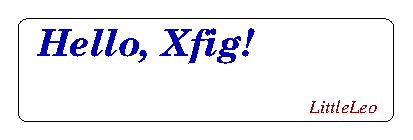
\includegraphics{hello}
  \caption{利用 Xfig 制图}
  \label{fig:xfig1}
\end{figure}

大学之道,在明明德,在亲民,在止于至善。知止而后有定;定而后能静;静而后能安;安
而后能虑;虑而后能得。物有本末,事有终始。知所先后,则近道矣。古之欲明明德于天
下者,先治其国;欲治其国者,先齐其家;欲齐其家者,先修其身;欲修其身者,先正其心;
欲正其心者,先诚其意;欲诚其意者,先致其知;致知在格物。物格而后知至;知至而后
意诚;意诚而后心正;心正而后身 修;身修而后家齐;家齐而后国治;国治而后天下
平。自天子以至于庶人,壹是皆以修身为本。其本乱而未治者 否矣。其所厚者薄,而其所
薄者厚,未之有也!

\hfill \pozhehao《大学》


\subsubsection{多个图形}
\label{sec:multifig}

如果多个图形相互独立,并不共用一个图形计数器,那么用 \verb|minipage| 或者
\verb|parbox| 就可以。否则,请参看图~\ref{fig:big1-subcaptionbox},它包含两个小图,分别是图~\ref{fig:subfig1} 
和图~\ref{fig:subfig2}。推荐使用\verb|\subcaptionbox|,
因为可以像图~\ref{fig:big1-subcaptionbox} 那样对齐子图的标题,
也可以使用\textsf{subcaption}宏包的\verb|\subcaption|(放在minipage中,用法同\verb|\caption|)
或是 subfigure 、 subtable环境,像图~\ref{fig:big1-subfigure},不要再用 \verb|\subfloat|、
\verb|\subfigure| 和 \verb|\subtable|。
\begin{figure}[h]
  \centering%
  \subcaptionbox{第一个小图形\label{fig:subfig1}}
  [3cm] %标题的长度,超过则会换行,如下一个小图。
    {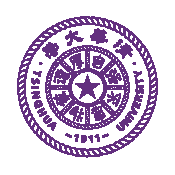
\includegraphics[height=3cm]{thu-fig-logo}}
      \hspace{4em}%
  \subcaptionbox{第二个小图形,注意这个图略矮些。如果标题很长的话,它会自动换行\label{fig:subfig2}}
      {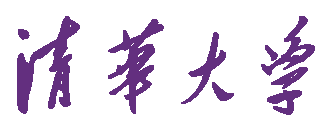
\includegraphics[height=2cm]{thu-text-logo}}
  \caption{包含子图形的大图形(subcaptionbox示例)}
  \label{fig:big1-subcaptionbox}
\end{figure}
\begin{figure}[h]
  \centering%
  \begin{subfigure}{3cm}
    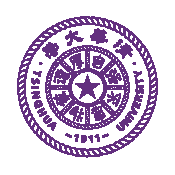
\includegraphics[height=3cm]{thu-fig-logo}
    \caption{第一个小图形}
  \end{subfigure}
  \hspace{4em}%
  \begin{subfigure}{0.5\textwidth}
    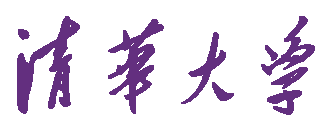
\includegraphics[height=2cm]{thu-text-logo}
    \caption{第二个小图形,注意这个图略矮些。subfigure中同一行的子图在顶端对齐。}
  \end{subfigure}
  \caption{包含子图形的大图形(subfigure示例)}
  \label{fig:big1-subfigure}
\end{figure}
古之学者必有师。师者,所以传道受业解惑也。人非生而知之者,孰能无惑?惑而不从师,
其为惑也,终不解矣。生乎吾前,其闻道也固先乎吾,吾从而师之;生乎吾後,其闻道也亦
先乎吾,吾从而师之。吾师道也,夫庸知其年之先後生於吾乎!是故无贵无贱无长无少,道
之所存,师之所存也。

嗟乎!师道之不传也久矣,欲人之无惑也难矣。古之圣人,其出人也远矣,犹且从师而问焉;
今之众人,其下圣人也亦远矣,而耻学於师。是故圣益圣,愚益愚。圣人之所以为圣,愚
人之所以为愚,其皆出於此乎?爱其子,择师而教之,於其身也,则耻师焉,惑焉。彼童子
之师,授之书而习其句读者,非吾所谓传其道、解其惑者也。句读之不知,惑之不解,或师
焉,或不焉,小学而大遗,吾未见其明也。巫医、乐师、百工之人不耻相师,  士大夫之族
曰“师”曰“弟子”之云者,则群聚而笑之。问之,则曰:彼与彼年相若也,道相似也,位
卑则足羞,官盛则近谀。呜呼!师道之不复,可知矣。巫医、乐师、百工之人。吾子不齿,
今其智乃反不能及,其可怪也欤!圣人无常师。孔子师郯子、苌子、师襄、老聃。郯子之徒,
其贤不及孔子。孔子曰:“三人行,必有我师。”是故弟子不必不如师,师不必贤於弟子。
闻道有先後,术业有专攻,如是而已。

如果要把编号的两个图形并排,那么小页就非常有用了:
\begin{figure}
\begin{minipage}{0.48\textwidth}
  \centering
  
\includegraphics[height=2cm]{thu-whole-logo}
  \caption{并排第一个图}
  \label{fig:parallel1}
\end{minipage}\hfill
\begin{minipage}{0.48\textwidth}
  \centering
  
\includegraphics[height=2cm]{thu-whole-logo}
  \caption{并排第二个图}
  \label{fig:parallel2}
\end{minipage}
\end{figure}

李氏子蟠,年十七,好古文、六艺,经传皆通习之,不拘於时,学於余。余嘉其能行古
道,作师说以贻之。

\hfill \pozhehao 韩愈(唐)



\chapter{背景}
\label{chapter:background}

\section{引言}
\label{section:background-introduction}

\section{突触模型}
\label{section:background-synapse-model}

\section{论文概要}
\label{section:background-outline}
%\chapter{回顾}
\label{chapter:review}

\section{非同步递质释放的生物机制}
\label{section:review:vesicle-release-mechanism}

\section{神经元突触的计算模型}
\label{section:review:neural-computation-model}

\section{总结}
\label{section:review:summary}
\chapter{计算模型}
\label{chapter:model}

\section{神经元模型}
\label{section:model:neuron-model}

常见的神经元模型包括 Hodgkin-Huxley 模型和 Integrate-and-Fire 模型。
前者可以模拟细胞膜上各种离子通道,通过调整参数,可以模拟出大量的特性。
后者不模拟离子通道的细节,只模拟细胞膜电位的变化,计算更高效。
介于两只之间的有 Izhikevich 模型,模型的部分参数失去了直观的物理意义,但通过调整参数,可以模拟出很多典型的神经元发放特性,同时计算也比 Hodgkin-Huxley 模型高效很多 \cite{Izhikevich2003,Izhikevich2004}。

\subsection{Izhikevich 模型}
Izhikevich 模型的动力学方程如下
\begin{align}
C \frac{\dd{v}}{\dd{t}} &= k \left( v-v_\text{r} \right) \left( v-v_\text{t} \right) - u + I \label{equation:izhikevich-membrane} \\
\frac{\dd{u}}{\dd{t}} &= a \left\{ b \left( v-v_\text{r} \right) - u \right\} \label{equation:izhikevich-recovery-current} \\
\text{当} v \geq v_{\text{peak}} \text{时,} & v \leftarrow c, u \leftarrow u + d \label{equation:izhikevich-spike}
\end{align}
其中 $v$ 是细胞膜电位, $u$ 是恢复电流, $C$ 是细胞膜电容, $v_\text{r}$ 是细胞膜静息电位, $v_\text{t}$ 是细胞膜自主发放电位。
$a$, $b$, $c$, $d$,和 $k$是其他参数, $I$ 是外部输入的电流。

在模拟快速发放神经元时,对模型中的式\ref{equation:izhikevich-recovery-current}进行一些改动,
\begin{align}
\frac{\dd{u}}{\dd{t}} &= 0.2 \left\{ U\left( v \right) - u \right\} \label{equation:izhikevich-fast-spiking} \\
U\left( v \right) &= \begin{cases} 0, &\mbox{当} v < v_\text{b} \mbox{时} \\ 0.025, &\mbox{当} v \geq v_\text{b} \mbox{时} \end{cases}
\end{align}
各项参数为
\begin{align*}
C &= 20\ \text{pF}, \\
k &= 1\ \text{pA} \cdot \text{mV$^{-2}$}, \\
v_\text{r} &= -55\ \text{mV}, \\
v_\text{t} &= -40\ \text{mV}, \\
v_\text{b} &= -55\ \text{mV}, \\
v_\text{peak} &= 25\ \text{mV}, \\
c &= -45\ \text{mV}.
\end{align*}

\section{突触模型}
\label{section:model:synapse-model}
流行的描述突触动态性的模型有 Misha Tsodyks 和 Henry Markram 提出的短时程突触可塑性(Short-Term Synaptic Plasticity)模型\cite{Markram1996,Tsodyks1997}。
最新版本的模型如下\cite{Tsodyks2013}

\begin{align}
\frac{\dd{u\left(t\right)}}{\dd{t}} &=  -\frac{u\left(t\right)}{\tau_f}+U\left[1-u\left(t\right)\right]\sum_m \delta\left(t-t_m\right), \label{equation:stp-facilitation} \\
\frac{\dd{x\left(t\right)}}{\dd{t}} &=
\frac{X_F-x\left(t\right)}{\tau_d} - q(t),
\label{equation:stp-depression} \\
q(t) & = u\left(t_+\right)x\left(t_-\right) \sum_m \delta\left(t-t_m\right),
\label{equation:stp-release}
\end{align}
其中 $u$ 代表细胞膜内钙离子残余造成的递质释放概率提升, $x$ 代表剩余的可释放递质的量, $q$ 代表递质的释放速率。 
$X_F$ 是静息状态下突触的可释放递质的总量。 
$\tau_f$, $U$, $\tau_d$ 是其他参数。不同类型的神经元有不同的参数 \cite{Silberberg2005}。

释放出的递质 $q$ 与突触后神经元上的递质接收器结合,产生突触后神经元细胞膜电流等一系列变化。
这部分也可以用模型描述\cite{Destexhe1994}。
\begin{align}
I_\text{syn}(t) &= g(t)\left(v(t) - E_\text{syn}\right), \label{equation:synaptic-current-general} \\
\frac{\dd{g(t)}}{\dd{t}} &= -\frac{g(t)}{\tau_\text{syn}} + wq(t - t_\text{delay}), \label{equation:receptor-conductance-general}
\end{align}
其中 $v$ 是突触后细胞的膜电位, $g$ 是离子通道的电导, $E_\text{syn}$ 是离子的反转电位, $w$ 是突触权重, $t_\text{delay}$ 是由于递质传递造成的延迟。

\subsection{非同步递质释放模型}
\label{section:model:asynchronous-release}
基于短时程突触可塑性模型,我们提出非同步递质释放模型,在原模型的基础上,增加非同步释放机制。
基于囊泡上存在两类不同特性的钙离子感受器,我们将式\ref{equation:stp-facilitation}分成两个形式一致,但具有不同参数的过程。
\begin{align}
\frac{\dd{u_\text{sr}\left(t\right)}}{\dd{t}} &= -\frac{u_\text{sr}\left(t\right)}{\tau_\text{sr}}+U_\text{sr}\left[1-u_\text{sr}\left(t\right)\right]\sum_m \delta\left(t-t_m\right), \label{equation:sr-facilitation} \\
\frac{\dd{u_\text{ar}\left(t\right)}}{\dd{t}} &= -\frac{u_\text{ar}\left(t\right)}{\tau_\text{ar}}+U_\text{ar}\left[1-u_\text{ar}\left(t\right)\right]\sum_m \delta\left(t-t_m\right), \label{equation:ar-facilitation}
\end{align}
其中 $u_\text{sr}$ 和 $u_\text{ar}$ 是由于钙离子结合造成的同步释放与非同步释放的不同的激活程度。
$U_\text{sr}$ 和 $U_\text{ar}$ 控制每个动作电位之后同步释放与非同步释放激活程度的提升大小。
$\tau_\text{sr}$ 和 $\tau_\text{ar}$ 控制钙离子感受器与钙离子分离造成同步释放与非同步释放激活程度下降的速度。

由于有实验支持同步释放和非同步释放竞争同一个递质资源池\cite{Otsu2004,Wen2010},所以使用单个变量 $x$ 来代表剩余的递质量,依旧沿用式\ref{equation:stp-depression}。

沿用原模型里的描述,只有动作电位到达后的短暂时刻有同步释放,同步释放的释放率为
\begin{equation}
q_\text{sr}(t) = u_\text{sr}(t_+)x(t_-)\sum_m \delta(t-t_m). \label{equation:sr-release}
\end{equation}

非同步释放则是高度随机的事件。
随机性使用二项过程模拟 \cite{DELCASTILLO1954}。
随机变量 $n$ 服从二项分布, $n\sim{\cal{B}}\left(N,p\right)$, 则它的概率分布函数为 $P(n=k|N,p) = \binom{N}{k} p^k (1-p)^{N-k}$, 其中 $k\in\{0,\ldots,N\}$, 且 $p$ 是单个事件发生的概率。

假设每个囊泡所含递质量相同,记为释放量子 $x_0$ ,那么在时刻 $t$ 剩余的可以释放的囊泡数量则有 $\sim \left\lfloor x(t)/x_0 \right\rfloor$ ,其中 $\lfloor \cdot \rfloor$ 表示取向下取整函数,取不大于自变量的最大整数。
在一个小的时间段 $[t,t+\dd{t})$ 内,单个囊泡由于非同步释放的钙离子感受器激活导致释放的释放概率为 $u_\text{ar}(t)\dd{t}$ ,$\dd{t}$ 取毫秒单位下的数值。
那么,非同步释放事件发生的数量 $n(t)$ 服从二项分布 ${\cal{B}}\left(\left\lfloor x(t)/x_0\right\rfloor,u_\text{ar}(t)\dd{t}\right)$。
因此,在时间段 $[t,t+\dd{t})$ 内释放的递质量为
\begin{equation}
  q_\text{ar}(t)\dd{t} = x_0 n(t), \label{equation:ar-release}
\end{equation}
其中 $n(t)$ 是上文定义的二项随机数。

在计算某段时间内同步释放与非同步释放的总和时,需要注意有些囊泡上可能同步释放和非同步释放的钙离子感受器同时激活,这部分递质量不应该被重复累加。
当时间段 $[t,t+\dd{t})$ 内发生了同步释放时,即有动作电位在这一时间段内到达,这部分同步释放和非同步释放的钙离子感受器同时激活导致的递质释放量为
\begin{equation}
q_\text{s\&a}(t)\dd{t} = q_\text{ar}(t)\dd{t}u_\text{sr}(t_+).
\end{equation}
如果在这一时间段内没有动作电位到达,那么 $q_\text{s\&a}(t) = 0$ 。

综上, $t$ 时刻总的递质释放率为
\begin{equation}
q(t) = q_\text{ar}(t) +q_\text{sr}(t) - q_\text{s\&a}(t). \label{equation:total-release}
\end{equation}

式\ref{equation:sr-facilitation},\ref{equation:ar-facilitation},\ref{equation:stp-depression},和\ref{equation:total-release}描述了扩展后模型的突触动力学。图\ref{figure:model-diagram}为模型的示意图。

\begin{figure}
\centering
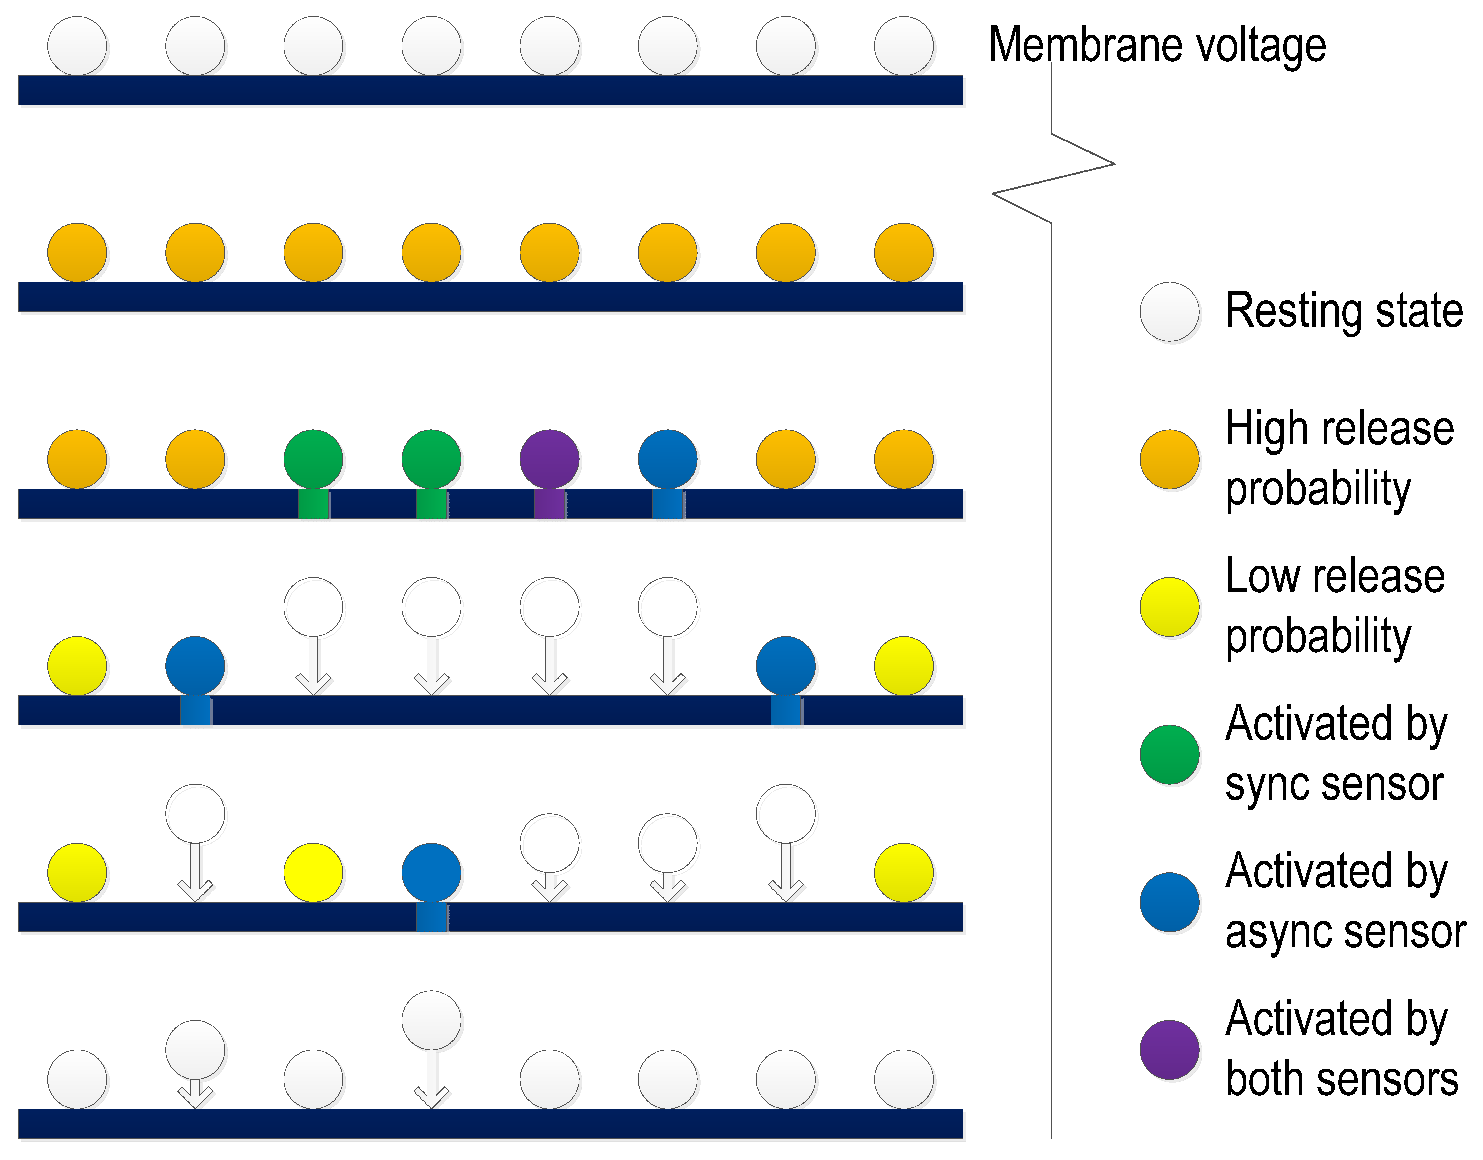
\includegraphics[scale=0.5]{model-diagram.eps}
\caption{同步释放与非同步释放突触模型示意图。描述突触从静息状态,到遇到动作电位,再回到静息状态的时间过程中各个阶段的变化。
第一行:突触处于静息状态,囊泡停泊在细胞膜上的活动区,准备释放,与囊泡上的钙离子感受器结合的钙离子较少,囊泡激活程度极低(用白色表示)。
第二行:一个动作电位过后,钙离子大量进入细胞内,与囊泡上的钙离子感受器结合,此时囊泡有较高的释放概率(用橙色表示)。
第三行:紧接着动作电位结束,一些囊泡被钙离子感受器激活(标记为绿色,蓝色,和紫色),开始与细胞膜融合并释放递质。这些囊泡有的是被同步释放的钙离子感受器激活(用绿色表示),有的是被非同步释放的钙离子感受器激活(用蓝色表示),还有的是两种钙离子感受器同时激活(用紫色表示)。
第四行:囊泡释放后细胞会新合成一些来补充到活动区(用箭头表示),在完成停泊上细胞膜之前这些囊泡无法释放。由于细胞内的钙离子清除机制,钙离子浓度会下降,剩余的可以释放的囊泡的释放概率降低。但仍有一些可以进行非同步释放(用蓝色表示)。
第五行:随着囊泡释放概率的降低,被非同步释放的钙离子感受器激活的囊泡越来越少。
第六行:钙离子浓度回到静息状态,等待下一个动作电位。}
\label{figure:model-diagram}
\end{figure}

\section{网络模型}
\label{section:model:network-model}
网络模型使用 Izhikevich 神经元模型,与带有非同步释放特性的突触模型结合组成抑制性快速发放神经元网络。
总共取 $n$ 个神经元,神经元之间随机链接,连接概率为 $p$。

在传统突触模型中,突触的状态可以由突触前神经元的发放完全决定,与突触后神经元无关。
这样由同一个神经元发出的多条突触的状态应该是完全相同的,仿真计算时只需模拟其中一条突触就可以了,计算量只会随着神经元数目 $n$ 的增多而线性增长 $O(n)$。

扩展后的非同步释放突触模型,即使不考虑突触后神经元对突触参数的影响,即同一个神经元发出的多条突触应该有相同的参数(不包括连接权重 $w$ ),状态也不会完全相同。
这是由于递质释过程放中存在随机性,假如所有突触的释放随机性是独立的,那么这些突触就会有不同的状态。
因此,仿真计算时每一条突触都需要单独模拟,计算量就会随着神经元数目 $n$ 的增加而平方级增长 $O(p \cdot n^2)$。


\section{简化模型}
\label{section:model:simplified-model}
某些情况下可以通过修改模型来减少计算量,提高计算速度。

\subsection{均匀释放模型}
扩展模型中非同步释放采用量子化的释放,这引入了随机性,如果放弃量子化释放,而按平均释放率进行释放,就可以消除随机性。
这需要把式\ref{equation:ar-release}
修改为

\begin{equation}
q_\text{ar}(t) = x(t) u_\text{ar}(t)\dd{t}
\label{equation:ar-release-simplified}
\end{equation}

这样,同一个神经元所发出的突触状态就完全一样,计算的复杂度又重新变回了 $O(n)$。

\subsection{随机相关释放}
均匀释放模型减小了递质释放的随机性。另一种简化策略是保留量子化随机释放,但同一个神经元发出的突触状态保持一致,即拥有完全相同的随机性。
这样可能会放大单个突触的释放随机性对整个网络的影响。

\chapter{研究材料与研究方法}
\label{chapter:methods}

我们提出了含有非同步释放的突触模型后,先基于实验数据对模型参数进行拟合,再进行仿真实验。

\section{实验材料}
\label{section:methods:materials}

用于参数拟合的实验数据来自前人实验里快速发放神经元的突触数据,数据采集的更多细节可以参考原始实验文献\cite{Jiang2012}。

\section{分析方法}
\label{section:methods:methods}

我们先对实验数据进行预处理,得到相关的统计信息,然后进行模型的参数拟合。

\subsection{数据预处理}
\label{section:methods:data-preprocessing}

\subsubsection{估计突触电流}
实验记录到的细胞膜电流包括细胞膜的漏电流 $I_\text{leaky}(t)$ 和由于突触信号传递导致的突触电流 $I_\text{syn}(t)$ 。

细胞产生漏电流的离子通道一般是受细胞膜电位调控的,实验条件下细胞膜电位被固定,可以假设漏电流恒定不变。
通过读取突触前细胞发放前一小段时间内突触后神经元的细胞膜电流,通过计算平均值可以得到漏电流 $I_\text{leaky}$ 。
记录的电流减去漏电流 $I_\text{leaky}$ 就能得到突触电流 $I_\text{syn}(t)$ 。
对于抑制性神经元的突触,它所产生的突触电流应该为非正值,但由于噪声的存在,可能有部分时间点 $t$ 时 $I_\text{syn}(t) > 0$。
这时需要对数据进行修正,先取一个极小的电流 $\epsilon > 0$ 作为阈值,对于 $I_\text{syn}(t) > -\epsilon$ 的时间点,将 $I_\text{syn}(t)$ 修改为 $-\epsilon$。
为了不引入太大的偏差, $\epsilon$ 需要足够小。
试验中取了 $\epsilon = 0.2$ pA,相对于IPSC的大小,这是一个非常小的值。

\subsubsection{去卷积方法}
根据突触后模型式\ref{equation:synaptic-current-general}和式\ref{equation:receptor-conductance-general},假设突触后神经元细胞膜电位为常数,则 $I_\text{syn}$ 可以表示成卷积的形式
\begin{equation}
I_\text{syn}(t) = \int_{-\infty}^t e^{-\frac{t - t'}{\tau_\text{GABA}}} A q(t' - t_\text{delay}) \dd{t'}
\label{equation:synaptic-current-convolution}
\end{equation}
其中 $A = w(v - E_\text{GABA})$。
实验条件下, $v$ 是稳定的常数,$E_\text{GABA}$ 在细胞处于平衡态时也应该是一个稳定的常数,因此可以假设实验中的递质释放率 $q(t)$ 和 突触电流 $I_\text{syn}$ 有式\ref{equation:synaptic-current-convolution}中的关系。
由于 $w$ 和 $E_\text{GABA}$ 是未知常数,所以 $A$ 也是未知常数,根据 $I_\text{syn}$ 最终只能得到 $Aq(t)$。

理论上可以使用傅里叶变换来曲卷积,得到估计的释放率 $q_e(t)$。
由于
\begin{equation}
I_\text{syn} = A \cdot K * q
\label{equation:synaptic-current-convolution-theory}
\end{equation}
其中 $K(t) = \cdot e^{-\frac{t}{\tau_\text{GABA}}}$, $*$ 表示卷积。
对式\ref{equation:synaptic-current-convolution-theory}进行傅里叶变换得到
\begin{equation}
F(I_\text{syn}) = A \cdot F(K) \cdot F(q)
\label{equation:synaptic-current-fourier-transformation}
\end{equation}
$F(f)$ 表示函数 $f$ 的傅里叶变换。
因此可以得到
\begin{equation}
A \cdot F(q) = \frac{F(I_\text{syn})}{F(K)}
\label{equation:release-rate-fourier}
\end{equation}
进行逆变换则可得到
\begin{equation}
A \cdot q = F^{-1}\left( F(I_\text{syn}) / F(K) \right)
\end{equation}

但实际试验中,由于IPSC的波形中高频傅里叶分量不可忽略,进行离散傅里叶变换会造成较大的误差。
即
\begin{equation}
\left| I_\text{syn} - A \cdot K * q_e \right| \gg 0
\label{equation:deconvolution-error}
\end{equation}

另一种通用的去卷积方法(MATLAB中的deconv函数)得到的 $q_e$ 波动剧烈且有大量 $q_e(t) < 0$ 的点存在。

因此在分析数据时使用了自己提出的曲卷积方法,此方法利用了式\ref{equation:synaptic-current-convolution-theory}中 $K$ 的特点,理论上只对指数衰减型的 $K$ 适用。
虽然降低了通用性,但能够避免前两种方法的缺点。

从试验记录中预处理得到的 $I_\text{syn}$ 的时间分辨率为 $\dd{t} = 0.05$ ms。
可将时间段 $[0, T]$ 分为 $N = T/\dd{t}$ 个宽度为 $\dd{t}$ 的小区间。
在离散形式下,第 $i$ 个时间区间内的突触电流为
\begin{equation}
I_\text{syn}(i) = \sum_{j=1}^i K(i-j)q(j-\Delta)\dd{t}
\label{equation:synaptic-current-discrete-convolution} 
\end{equation}
其中当 $i \geq j$ 时,$K(i-j) = Ae^{-(i-j)\dd{t}/\tau_\text{GABA}}$,当 $i < j$ 时,$K(i-j) = 0$,$\Delta = t_\text{delay}/\dd{t}$。

首先,通过确定 GABA 递质接收器的衰减常数 $\tau_\text{GABA}$ 来确定 $K$。
使用 MATLAB 的 Curve Fitting Toolbox。
拟合的目标函数为 $\text{fittype}(@(A, t_0, \tau, leaky, t) A .* exp(-(t-t_0)/\tau) .* (t > t_0) + leaky)$。
表示
\begin{equation}
I_\text{syn}(t) = 
\begin{cases}
A \cdot e^{-(t-t_0)/\tau_\text{GABA}} + I_\text{leaky}, & \text{若 } t > t_0 \\
I_\text{leaky}, & \text{若 } t \leq t_0
\end{cases}
\end{equation}

通过分析自发释放和单个动作电位导致的释放,得到突触的参数 $\tau_\text{GABA}$。
对于快速发放神经元到快速发放神经元的突触, $\tau_\text{GABA} \approx 2.6$ ms。
对于快速发放神经元到金字塔形神经元的突触, $\tau_\text{GABA} \approx 5$ ms (见图\ref{figure:decay-time-constant})。
这与之前文献的记录相符\cite{Bartos2002}。

\begin{figure}
\centering
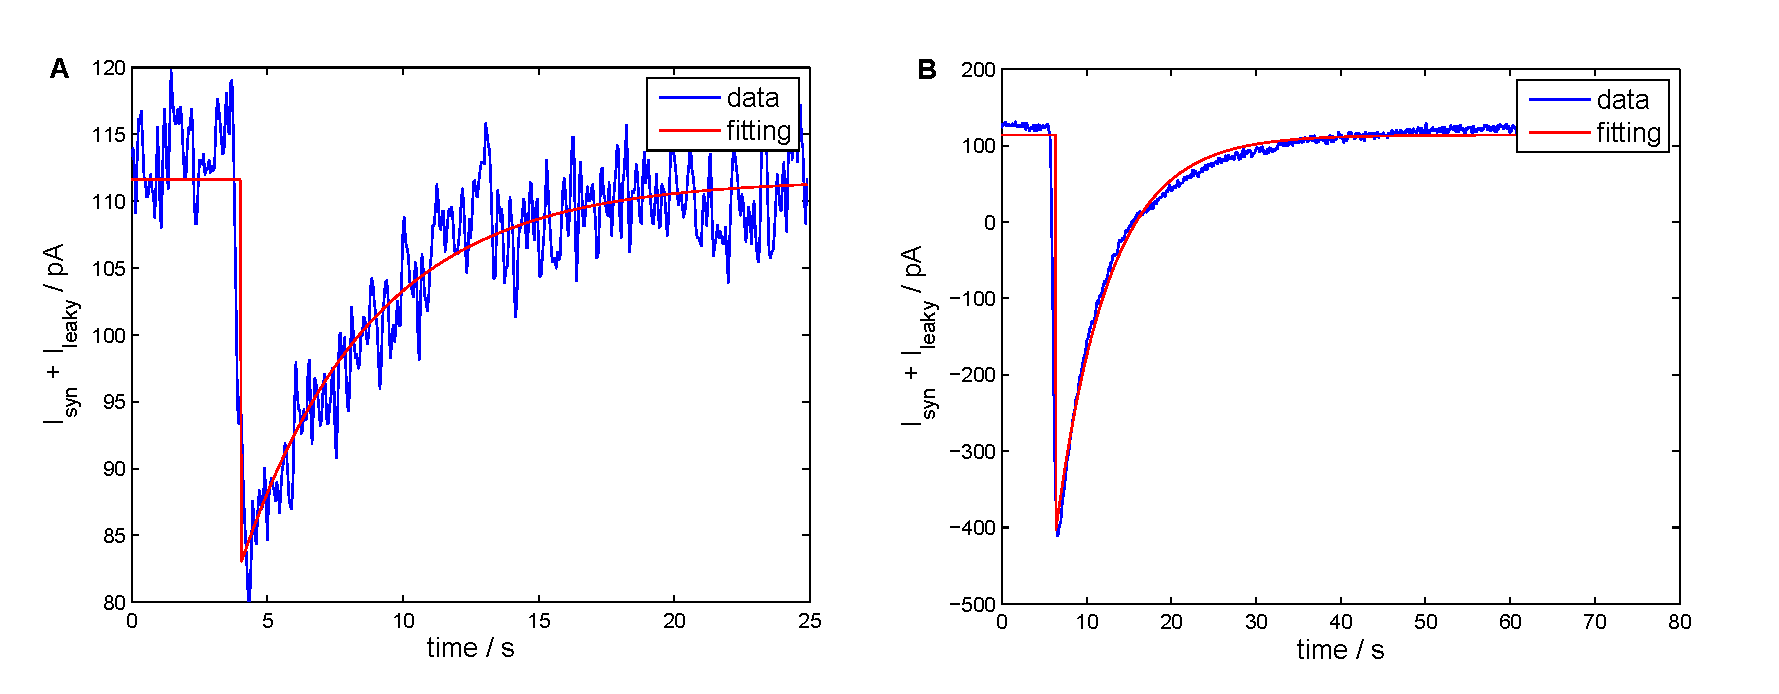
\includegraphics[scale=0.5]{fs-pc-decay-time-constant.eps}
\caption{拟合GABA递质接收器的衰减常数 $\tau_\text{GABA}$。实验数据来自癫痫病人的脑组织切片中快速发放神经元到金字塔形神经元的突触。蓝线表示实验记录的 IPSC ,红线为拟合的结果。
(A)为自发的递质释放,得到的估计值为 $\tau_\text{GABA} \approx 4.8$ ms (置信区间为 $4.39$ ms - $5.27$ ms)。
(B)为单个动作电位引发的递质释放,得到的估计值为 $\tau_\text{GABA} \approx 6.2$ ms (置信区间为 $6.06$ ms - $6.46$ ms)。}
\label{figure:decay-time-constant}
\end{figure}


得到了 $K$ 之后,使用贪心策略,一步一步递进得到 $Aq(i - \Delta)$ 对于 $i - \Delta = 1,2,\cdots,N$ 的所有值。
初始状态下 $Aq = 0$,在第 $i$ 步,假设 $q(j - \Delta)$ 在 $j = 1,2,\cdots,i-1$ 时已经得到估计值,此时我们选取 $q(i - \Delta)$ 为
\begin{equation}
\begin{split}
q(i - \Delta) &= \Argmin_{p \geq 0} \left| \sum_{j=1}^{i-1} K(i-j)q(j-\Delta)\dd{t} + Ap\dd{t} - I_\text{syn}(i) \right| \\
\text{且满足 } & \forall k \geq i, I_\text{syn}(k) \geq e^{-(k-i)\dd{t}/\tau_\text{GABA}} \cdot J(i)
\end{split}
\end{equation}
其中 $J(i) = \sum_{j=1}^{i-1} K(i-j)q(j-\Delta)\dd{t} + Ap\dd{t}$。
这样得到的估计值 $Aq_e(t - t_\text{delay})$ 满足 $A \cdot K * q_e \leq I_\text{syn}$。
约束条件 $\forall k \geq i, I_\text{syn}(k) \geq e^{-(k-i)\dd{t}/\tau_\text{GABA}} \cdot J(i)$ 保证了第 $i$ 步之后存在 $Aq \geq 0$ 的值满足$A \cdot K * q_e \leq I_\text{syn}$。

结果显示得到的 $Aq_e$ 进行卷积后与 $I_\text{syn}$ 非常接近(见图\ref{figure:deconvolution-and-latency}A-B)。
\begin{figure}
\centering
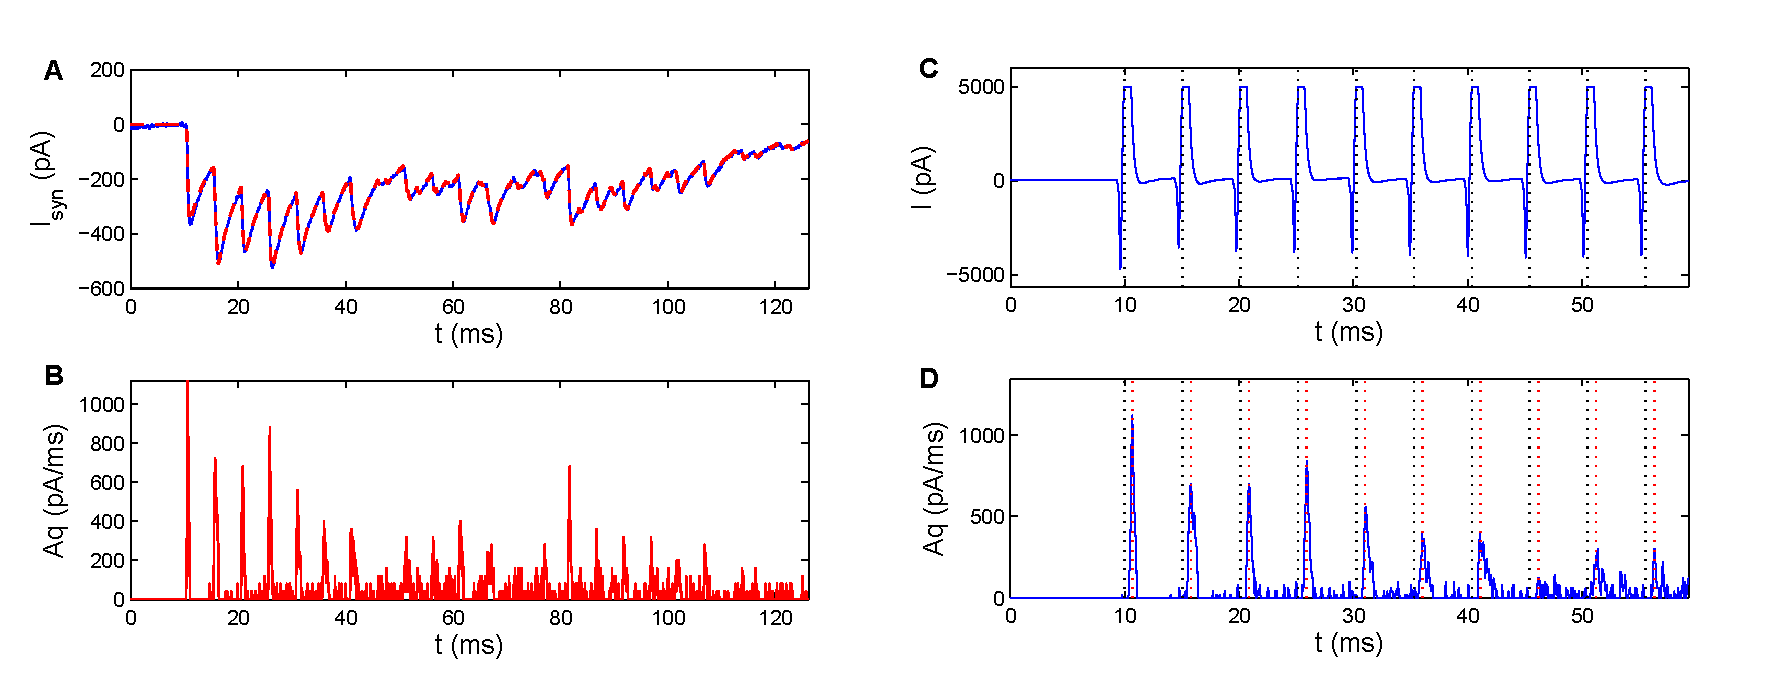
\includegraphics[scale=0.5]{fs-pc-deconvolution-and-latency.eps}
\caption{IPSC的去卷积。数据来自人类癫痫患者脑组织切片中快速发放神经元到金字塔形神经元的突触。
(A)蓝线为原始的一部分IPSC记录。红色虚线为基于 $Aq_e$ (来自B) 进行卷积后得到的结果。
两条曲线非常接近。
(B)根据实验数据分析出的IPSC(来自A)估计出的递质释放率 $\tilde{q} = Aq$。
(C-D)通过比较突触前神经元的发放时间(黑色虚线)和 $Aq(t-t_\text{delay}$ 的极高点得到 $t_\text{delay}$。
(C)突触前神经元的细胞膜电流,黑色虚线选择为神经元发放的时间。
(D)黑色虚线与 C 中时间一致,每个红色虚线比相应的黑色虚线晚 $0.75$ ms,与释放率的极高点大致重合。所以突触传递的延迟 $t_\text{delay}$ 约为 $0.75$ ms。
}
\label{figure:deconvolution-and-latency}
\end{figure}

\subsection{数据拟合}
\label{section:methods:data-fitting}
我们从实验数据中选取了 $n = 12$ 个记录得到了 $100$ Hz 频率发放动作电位时的递质释放率。
其中动作电位的发放次数分别为 $10$, $15$, $20$, 和 $25$,各有 $3$ 次重复实验。
为了便于比较,我们只选取前 $N_{sp} = 10$ 个动作电位的数据进行统计。

由于实验记录中噪声的存在,且非同步释放本身高度随机,所以这里通过将递质释放率分成多个时间区间分段统计平均释放率,并于模型进行比较,来确定模型的参数。

通过比较突触前神经元的细胞膜电流和估计出的释放率,我们观察到释放率的极高点相对于突触前神经元的发放大约总是落后 $t_\text{delay} = 0.75$ ms(见图\ref{figure:deconvolution-and-latency}C-D)。这个值就选取为式\ref{equation:receptor-conductance-general}中的突出传递延迟。

更多统计后发现,递质释放率在突触前神经元发放 $0.3$ ms 后开始急剧上升,持续约 $1.1$ ms 后急剧下降。
因此我们把时间分为两种区间。
第一种开始于突触前神经元每个动作电位后的 $0.3$ ms,持续 $1.1$ ms,这些区间记为同步释放区间 $P_\text{sr}^{(k,i)}$ ,表示第 $i$ 次试验中第 $k$ 个动作电位之后的同步释放区间。
第二种则是两个同步释放区间之间的时间段,记为非同步释放区间 $P_\text{ar}^{(k,i)}$。
神经递质在相应区间内的释放总量为
\begin{equation}
M_\text{r}^{(k,i)} = \int_{t \in P_\text{r}^{(k,i)}} Aq(t)\dd{t}
\end{equation}
其中 $\text{r} = \text{sr}, \text{ar}$。

得到了这些区间内的释放量后,我们采用概率推断的方法来估计模型参数,此方法与拟合 STP 模型用的某个方法类似\cite{Costa2013}。
这里同样假设某个特定释放区间内的递质释放量服从高斯分布。
因此我们只是用样本在多次实验记录中的均值和标准差来拟合模型。
\begin{align}
\mu_\text{r}^{(k)} &= \frac{1}{n} \sum_i M_\text{r}^{(k,i)} \\
\sigma_\text{r}^{(k)} &= \sqrt{\frac{1}{n}\sum_i\left( M_\text{r}^{(k,i)} - \mu_\text{r}^{(k)} \right)^2}
\label{equation:statistics-for-fitting}
\end{align}

根据定义的同步和非同步释放区间计算得到 $\bm{M_\text{r}}$ 之后,对于给定的参数组合 $\bm{\theta} = \{\tau_\text{sr}$,
$U_\text{sr}$, $\tau_\text{ar}$, $U_\text{ar}$, $\tau_d$, $X_F$, $x_0 \}$ 对实验观测 $\bm{M_\text{r}}$ 的似然度记为 $P\left(\bm{M_\text{r}}\left|\bm{\theta}\right.\right)$。

对于每一组参数 $\bm{\theta}$,相应的似然度为
\begin{equation}
 \log P\left(\bm{M_\text{r}}\left|\bm{\theta}\right.\right) = \sum_{r \in
    \{\text{sr}, \text{ar}\}}
  \sum_{k=1}^{N_{sp}} \left(-\frac{\big(\tilde{M}_{r}^{(k)}-\mu_{r}^{(k)}\big)^2}{2\big(\sigma_r^{(k)}\big)^2}
- \log\sqrt{2\pi}\sigma^{(k)} \right),
\label{equation:probabilistic-inference-log}
\end{equation}
其中 $\tilde{M}_\text{r}^{(k)}$ 计算模型在相应释放区间内的平均释放量。
此处取自然对数是为了防止数值计算时数值变化范围过大造成溢出。

由于式\ref{equation:ar-release}具有随机性,每一个时间区间内的 $\tilde{M}_\text{r}^{(k)}$ 需要多次计算取平均值。为了节省时间,我们将式\ref{equation:ar-release}简化为式\ref{equation:ar-release-simplified},即
\begin{equation*}
q_\text{ar}(t) = x(t) u_\text{ar}(t)\dd{t}
\end{equation*}
这样模型中就不再有随机性,一次计算就可以得到释放率的平均值。
这一改动同时使得 $x_0$ 变成了一个不起作用的参数,我们之后将用其他方法来估计 $x_0$ 的值。

我们得到了模型产生的释放率 $q'(t)$ 之后,用类似的方式计算模型的 $\tilde{M}_\text{r}^{(k)}$,此时同步释放区间 $P_\text{sr}^{(k,i)}$ 从发放时开始,持续 $1.1$ ms,,没有了延迟。
然后计算一个归一化参数 $A$,对应于 $w(v-E_\text{GABA})$,以此确保总释放量 $\sum \tilde{M}_\text{r}^{(k)}$ 与实验数据一致。

注意到递质的释放量与参数 $X_F$ 成正比 (根据式\ref{equation:sr-facilitation},式\ref{equation:ar-facilitation},式\ref{equation:total-release},和式\ref{equation:stp-depression}),即 $A \propto \frac{1}{X_F}$。这意味着如果不限定 $A$ 的值,就无法得到 $X_F$。因此不失一般性,在参数拟合过程中使用 $X_F = 1$。

通过网格式搜索来寻找使得似然度最大的参数组合。表\ref{table:parameters}中列出了搜索区间和推断出的结果。
\begin{table}
  \centering
  \begin{tabular}{llllll}
    \hline\hline
    & 参数 & 单位 & 值 & 搜索空间 & 置信区间 \\
    \hline
    & $U_\text{sr}$ & & $0.16$ & $[0.04, 0.40]$ & $[0.1550, 0.1605]$ \\
    & $\tau_\text{sr}$& ms & $1$ & $[1, 8]$ & $[0.10, 2.56]$ \\
    & $U_\text{ar}$ & & $0.020$ & $[0.008, 0.024]$ & $[0.0202, 0.0212]$ \\
    & $\tau_\text{ar}$ &ms & $8$ & $[4, 48]$ & $[8.022, 8.380]$ \\
    & $\tau_d$ &ms & $35$ & $[10, 100]$ & $[35.74, 39.04]$ \\
    & $X_F / x_0$& & $135$ & n.a. & n.a. \\
    \hline
\end{tabular}
\caption{网格式搜索寻找最大似然度参数组合的搜索区间和最终的搜索结果。此处 $\frac{X_F}{x_0}$ 是一个常数,表示在突触的活动区内最初的可以释放的囊泡数目。}
\label{table:parameters}
\end{table}

在找到了极优参数组合 $\bm{\hat{\theta}}$ 后,我们在参数组合的每一个维度,在更小的范围内用更密集的采样点来检查附近的参数。
每个维度的置信区间取似然度大于最大似然度 $90\%$ 的那些点。
表\ref{table:parameters}中有各维度的置信区间。

\begin{figure}
\centering
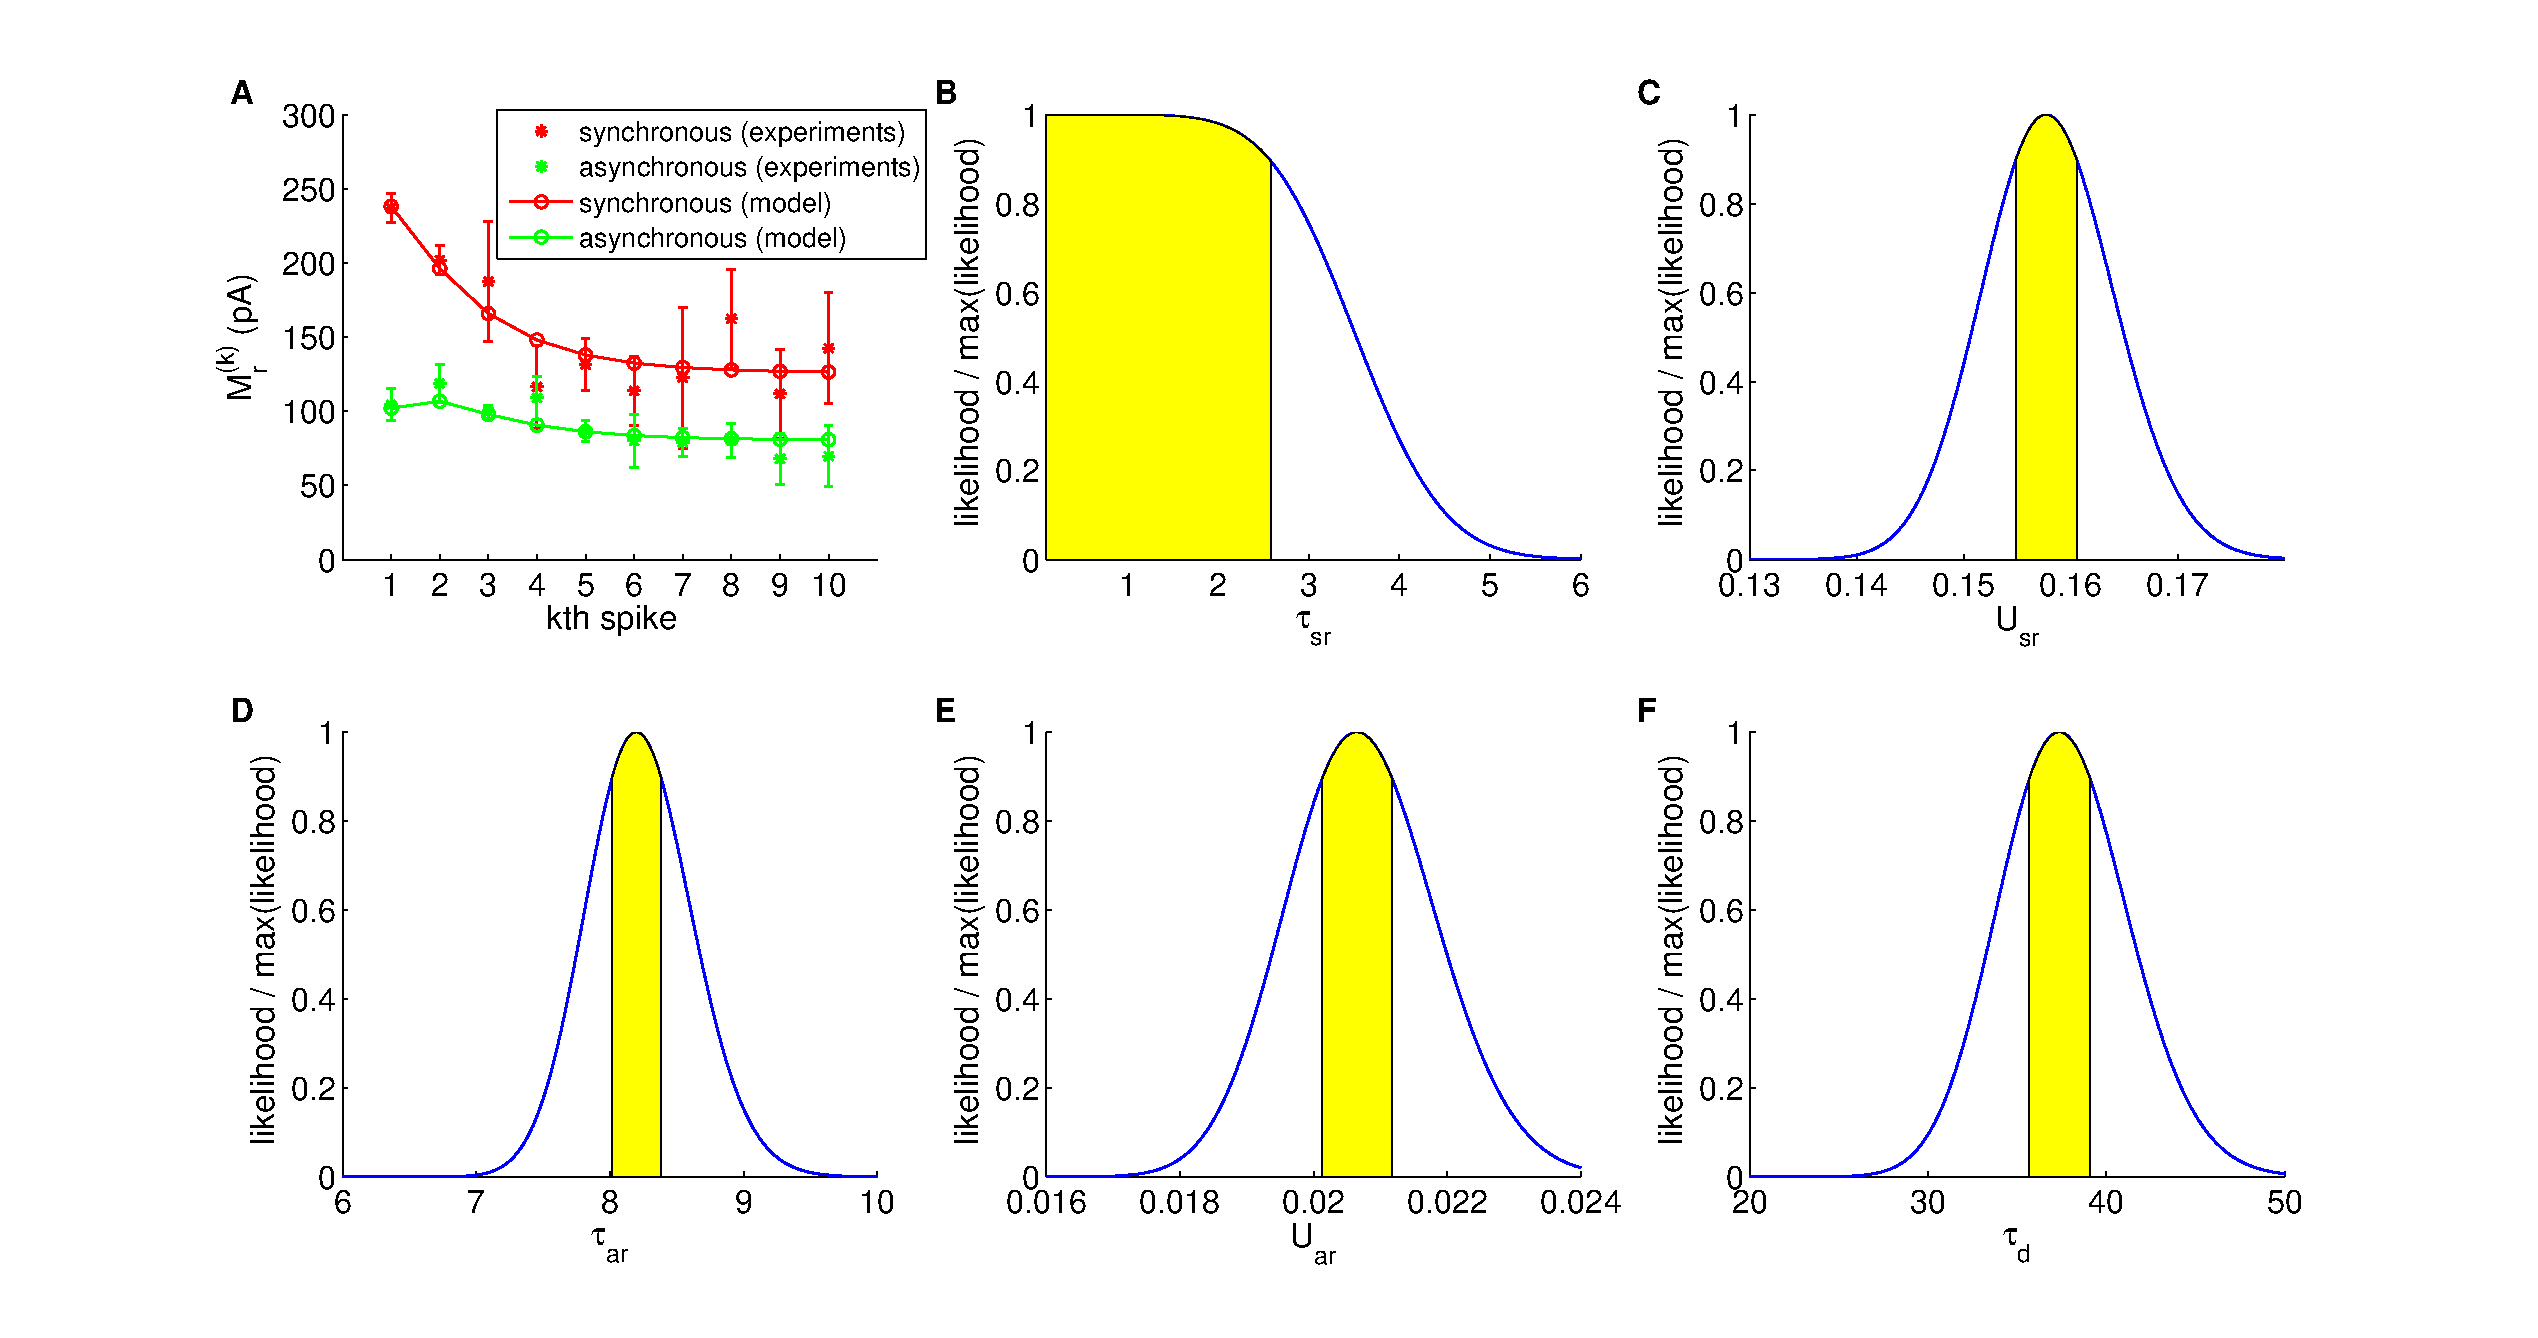
\includegraphics[scale=0.36]{fitting-results.eps}
\caption{模型参数拟合。
(A)第 $k$ 个动作电位后的平均释放量。*表示实验中统计的同步释放区间内的释放量(红色)和非同步释放区间内的释放量(蓝色)。误差棒表示标准差。实线为极优参数组合下的模型的统计数据。两者较一致。
(B-F)每个维度上在极优参数附近的置信区间。}
\label{figure:fs-pc-fitting}
\end{figure}

\subsubsection{计算囊泡释放量子}
在参数 $\tau_\text{sr}$,$U_\text{sr}$, $\tau_\text{ar}$, $U_\text{ar}$, $\tau_d$ 找到之后,我们就可以接着计算 $x_0$ 的大小。

\chapter{仿真计算结果}
\label{chapter:results}
在确定了仿真计算模型和相关参数后,接下来就要探索非同步释放对单个神经元和神经元网络的影响。

\section{模型参数}
\label{section:results:parameters}
从图\ref{figure:fs-pc-fitting}看出,模型能够与实验数据很好地拟合,默认情况下选用表\ref{table:parameters}中的最优参数进行仿真计算。

\section{通过调整模型参数模拟非同步释放的变化}
\label{section:result:modulate-asynchronous-release}
不同类型的类型的神经元能够具有不同的模型参数。
同一种类型的神经元,在不同的环境下也可能具有不同的模型参数。
接下来我们将展示不同参数的变化对突触的最终递质释放的影响。
为了使描述更加清晰,我们将同步释放与非同步释放造成的 IPSC 分别展示。
即,基于式\ref{equation:total-release},我们把 IPSC 分解为 $I_\text{sr}$ 和 $I_\text{ar}$
\begin{align}
I_\text{syn}(t) &= I_\text{sr}(t) + I_\text{ar}(t) \\
I_\text{sr}(t) &= \int_{-\infty}^t e^{-\frac{t - t'}{\tau_\text{GABA}}} w(v - E_\text{GABA})\left( q_\text{sr}(t') + q_\text{s\&a}(t') \right) \dd{t'} \\
I_\text{ar}(t) &= \int_{-\infty}^t e^{-\frac{t - t'}{\tau_\text{GABA}}} w(v - E_\text{GABA})q_\text{ar}(t') \dd{t'}
\end{align}

$\tau_\text{ar}$, $U_\text{ar}$ 和 $X_F / x_0$ 这三个参数直接影响非同步释放,以下将依次展现影响效果。

\subsection{模拟钙离子清除变慢导致的非同步释放增强}
\label{section:result:modulate-with-tau-ar}
对癫痫病人脑组织中的快速发放神经元进行参数拟合后发现,非同步释放的衰减常数为 $\tau_\text{ar} = 8$ ms (见表\ref{table:parameters}),这意味着神经元停止发放后非同步释放减弱速率很快。
前人的研究中发现,表达了 CCK 的神经元中发放停止后非同步释放的衰减速率较慢 \cite{Hefft2005}。
机制上,释放速率的快速降低可能是由于快速发放神经元细胞内包含的 PV 物质导致。
PV 是一种蛋白质,能够使自由钙离子浓度快速下降,导致钙离子感受器快速去激活。
因此 $\tau_\text{ar}$ 在包含 PV 的快速发放神经元中相对较小。
同时,前人的研究也发现钙离子的快速清除能够导致非同步释放减弱 \cite{Jiang2015}。

在实验中,经常使用 EGTA-AM 溶液浸泡来调节细胞内自由钙离子的清除速率。
增加 EGTA-AM 可以提高钙离子的清除 \cite{Otsu2004,Jiang2015}。
这种调控对应于模型中 $\tau_\text{sr}$ 与 $\tau_\text{ar}$ 的改变。
由于两类钙离子感受器具有不同的生物化学性质,所以同一操作对 $\tau_\text{sr}$ 和 $\tau_\text{ar}$ 能造成不同的影响。

我们调节 $\tau_\text{ar}$ 来展示这一参数对同步释放和非同步释放的影响。
将 $\tau_\text{ar}$ 从 $8$ ms 增大到 $30$ ms 能够使 $u_\text{ar}$ 衰减速率明显减缓,这样 $u_\text{ar}$ 就能够在持续发中积累并饱和在一个较高的水平,导致更大的 $I_\text{ar}$ (见图\ref{figure:modulation-of-tau-ar})。
此外,非同步释放增强导致可释放的递质资源 $x$ 变小,间接导致 $I_\text{sr}$ 减小。
这种形式的竞争现象在前人的实验中也有发现 \cite{Otsu2004}。
最终,在发放结束后,非同步释放的电流由于衰减变慢而持续时间更长。

 
\begin{figure}
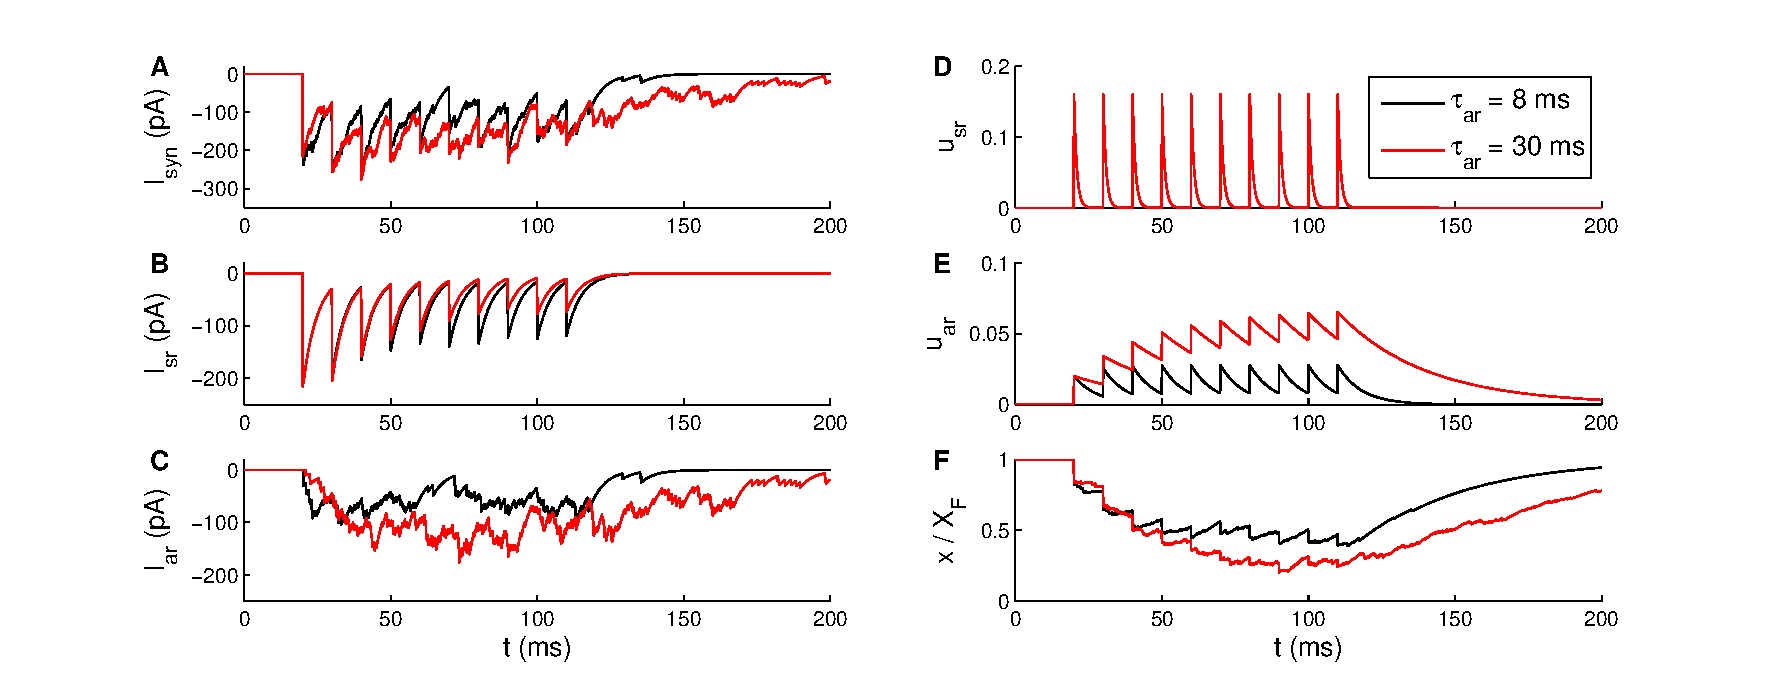
\includegraphics[scale=0.5]{sync-vs-async-ipsc-internals-tau-ar.eps}
\caption{模型中 $\tau_\text{ar}$ 对非同步释放的影响。
仿真计算使用表\ref{table:parameters}中的参数作为默认参数。
$\tau_\text{ar}$ 使用自定义的值,黑线对应 $\tau_\text{ar} = 8$ ms,红线对应 $\tau_\text{ar} = 30$ ms。
神经元发放开始于 $20$ ms,结束于 $110$ ms,发放频率为 $100$ Hz (每次共 $10$ 个动作电位)。
一个量子化释放导致的 IPSC 的高度为 $Ax_0 = 10$ pA。
(A) 总的递质释放导致的 IPSC。
(B) IPSC 中同步释放导致的部分。
(C) IPSC 中非同步释放导致的部分。
(D) 内部状态 $u_\text{sr}$。
(E) 内部状态 $u_\text{ar}$。
(F) 内部状态 $x$ (缩放比例为 $1:X_F$)。}
\label{figure:modulation-of-tau-ar}
\end{figure}


\subsection{模拟神经元动作电位变化导致的非同步释放变化}
\label{section:result:modulate-with-u-ar}
在大鼠的脑组织中发现,癫痫组织细胞的动作电位比正常组织细胞的更高 \cite{Jiang2012}。
理论上更高的动作电位会导致电压依赖的钙离子通道打开更大,使更多的钙离子流入细胞内,进而导致囊泡上的钙离子感受器激活程度更高。
调节动作电位的高度对非同步释放的影响大于同步释放 \cite{Jiang2012}。
流入的钙离子增多对应于模型中 $U_\text{sr}$ 和 $U_\text{ar}$ 的改变。

我们调节 $U_\text{ar}$ 来展示这一参数对同步释放和非同步释放的影响。
将 $U_\text{ar}$ 从 $0.02$ 增加到 $0.06$ 能够使 $u_\text{ar}$ 在每个动作电位后增长更高,由于 $\tau_\text{ar}$ 较小, $u_\text{ar}$ 在很少几个动作电位后会很快饱和。
更高的 $u_\text{ar}$ 导致更大的 $I_\text{ar}$ (见图\ref{figure:modulation-of-u-ar})。
与之前的仿真结果类似,非同步释放增强导致可释放的递质资源 $x$ 变小,间接导致 $I_\text{sr}$ 减小。
 
\begin{figure}
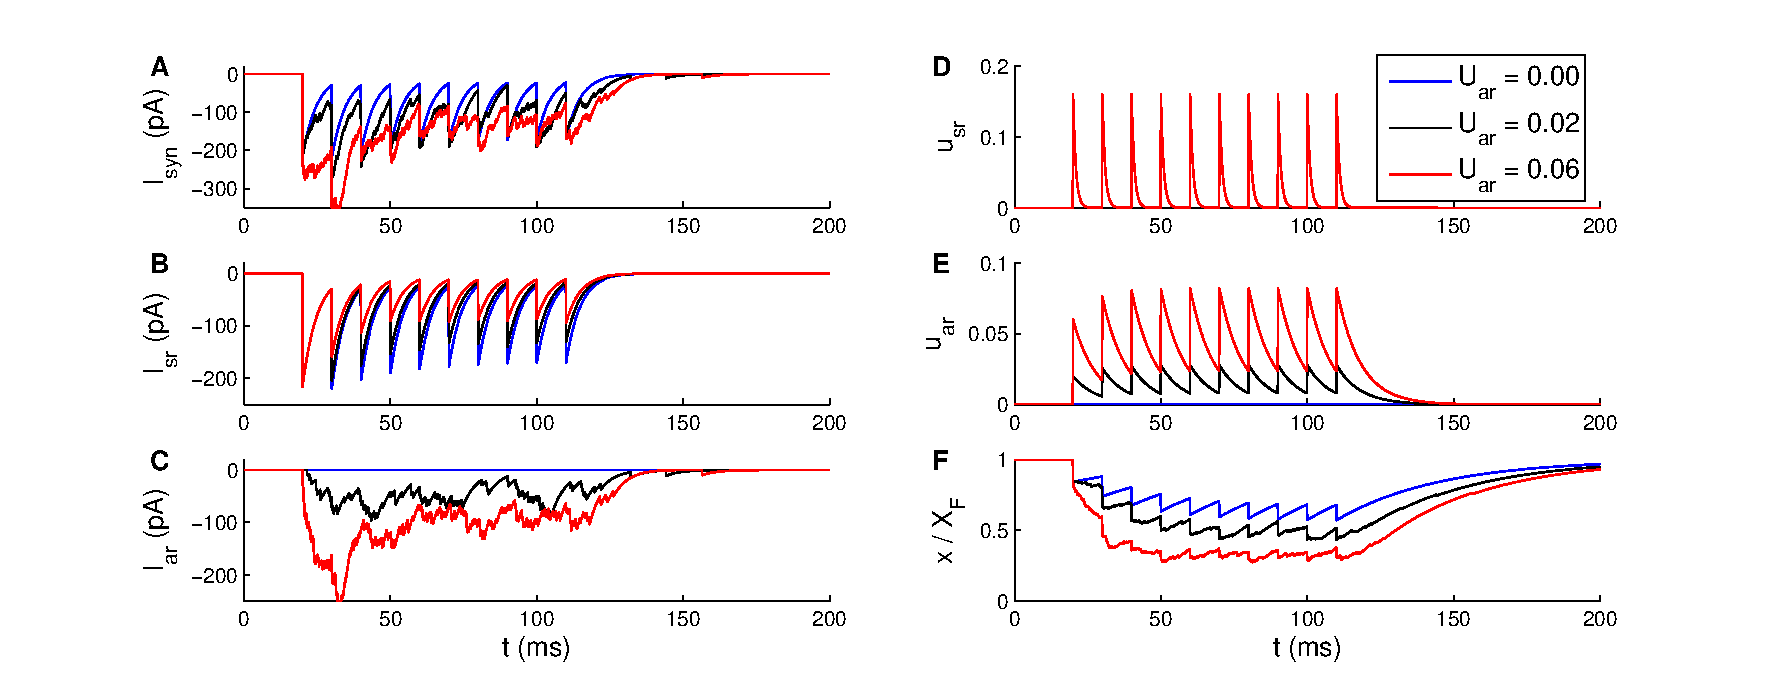
\includegraphics[scale=0.5]{sync-vs-async-ipsc-internals-u-ar.eps}
\caption{模型中 $\tau_\text{ar}$ 对非同步释放的影响。
仿真计算使用表\ref{table:parameters}中的参数作为默认参数。
$U_\text{ar}$ 使用自定义的值,蓝线对应 $U_\text{ar} = 0$,即没有非同步释放,黑线对应 $U_\text{ar} = 0.02$,红线对应 $U_\text{ar} = 0.06$。
神经元发放开始于 $20$ ms,结束于 $110$ ms,发放频率为 $100$ Hz (每次共 $10$ 个动作电位)。
一个量子化释放导致的 IPSC 的高度为 $Ax_0 = 10$ pA。
(A) 总的递质释放导致的 IPSC。
(B) IPSC 中同步释放导致的部分。
(C) IPSC 中非同步释放导致的部分。
(D) 内部状态 $u_\text{sr}$。
(E) 内部状态 $u_\text{ar}$。
(F) 内部状态 $x$ (缩放比例为 $1:X_F$)。}
\label{figure:modulation-of-u-ar}
\end{figure}

\subsection{模拟囊泡相对大小对突触后电流波动的影响}
\label{section:result:modulate-x-0}
我们发现改变 $x_0$ 的相对大小可以影响非同步释放的随机性大小。

假设可释放的递质总量一定,但每个囊泡包含了更少的递质(意味着囊泡数量增多)。
在模型中,保持 $wX_F$ 不变,同时通过减小 $x_0$ 来增加总共可用的囊泡数目 $\frac{X_F}{x_0}$,此处 $w$ 是突触模型中的突触权重(见式\ref{equation:receptor-conductance-general})。

假设在时刻 $t$,剩余递质的比例为 $\xi$。
那么此时共有 $\frac{\xi X_F}{x_0}$ 个囊泡,每一个囊泡在一小段时间内释放的概率都是 $p$,根据二项过程的性质,囊泡释放数量的方差为 $\frac{\xi X_F}{x_0}p(1-p)$。
那么对式\ref{equation:receptor-conductance-general}中的电导 $g$ 造成的方差为
\begin{equation}
\begin{split}
(wx_0)^2 \frac{\xi X_F}{x_0} p (1-p) &= wx_0 (\xi  w  X_F) p (1-p) \\
&= wx_0  c
\end{split}
\label{equation:quantum-effect}
\end{equation}
其中由于 $wX_F$ 保持为常数,故 $c$ 是常数。
因此,对于更大的 $X_F/x_0$, $wx_0$ 会更小,即有递质的随机释放导致的电导的方差更小。
更小的 $wx_0$ 会使非同步释放导致的 IPSC 更光滑(见图)。

\begin{figure}
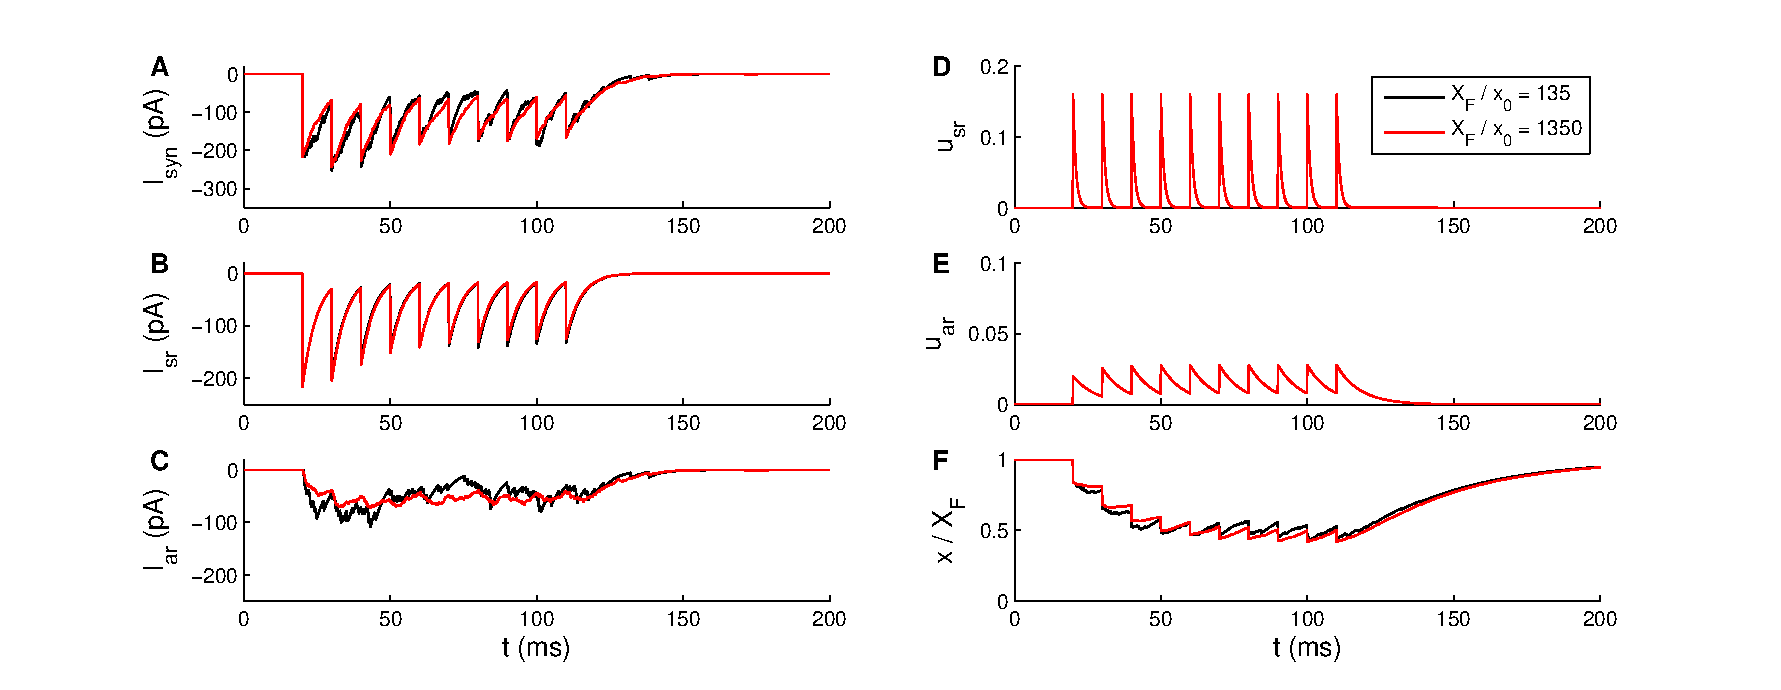
\includegraphics[scale=0.5]{sync-vs-async-ipsc-internals-x-0.eps}
\caption{释放量子大小在模型中对 IPSC 的影响。
黑线设置 $X_F / x_0 = 135$, $Ax_0 = 10$ pA,
红线设置 $X_F / x_0 = 1350$, $Ax_0 = 1$ pA,
其他参数使用表\ref{table:parameters}中的作为默认值。
(A) 总的递质释放导致的 IPSC。
(B) IPSC 中同步释放导致的部分。
(C) IPSC 中非同步释放导致的部分。
(D) 内部状态 $u_\text{sr}$。
(E) 内部状态 $u_\text{ar}$。
(F) 内部状态 $x$ (缩放比例为 $1:X_F$)。
可以明显看出更小的 $X_F/x_0$ 使得 IPSC 更光滑。}
\label{figure:changes-with-x-0} 
\end{figure}


\section{网络仿真计算}
\label{section:resutl:network}
神经元网络仿真计算选择让网络处于同步发放状态,基于此种状态展示非同步递质释放的影响。

神经元网络仿真计算采用 $n = 200$ 个神经元(模型见第\ref{chapter:model}章),突触包含非同步递质释放,突触后递质接收器模型为
\begin{align}
\label{equation:network-receptor-model}
\frac{\dd{g_i\left(t\right)}}{\dd{t}} &= - \frac{g_i\left(t\right)}{\tau_\text{GABA}} + w_i \cdot q_i\left(t - t_\text{delay}\right) \\
I_\text{syn} &= \sum_i g_i\left(v-E_\text{GABA}\right) \\
I &= - I_\text{syn} + I_\text{ext}
\end{align}
其中 $i$ 为神经元编号,$t_\text{delay} = 1$ ms,$E_\text{GABA} = -70$ mV。
$E(w_i) \approx \frac{w_0}{pn}$, $p$ 为链接概率。

为了使现象更明显,我们放宽了参数的选择范围。
\begin{align}
\label{equation:network-parameters}
\tau_\text{sr} &=  8 \ \text{ms} \\
\Delta U_\text{sr} &= 0.245 \\
\tau_\text{ar} &= 50 \ \text{ms} \\
\Delta U_\text{ar} &= 0.004 \\
\tau_d &= 110 \ \text{ms} \\
x_0/X_F &= 0.01 \\
X_F &= 1
\end{align}


\subsection{非同步释放对网络同步的影响}
\label{section:result:network-synchronization}
非同步释放具有更长的衰减常数,为了展示这一特性的影响,我们采用简化模型(式\ref{equation:ar-release-simplified}),这样递质的释放就变成了没有随机性的过程。
仿真结果显示非同步释放能使网络稳定在同相位状态,而同步释放促使我网络离开同相位状态,进入反相位状态。

模拟参数为 $\tau_\text{GABA} = 5$ ms,$w_0 = 35$ nS, $p = 1$。
网络包含非同步释放时有两种稳定状态——同相位和反相位。
由于非同步释放相对于同步释放较弱,所以同相位的状态转移势垒低于反相位。
网络进入哪一种状态与网络初始状态和背景输入有关(图\ref{figure:network-stability})。

图\ref{figure:network-stability}中每个字图的第一行为每个神经元发放时间的记录,第二行为一个小时间窗口内发放了的神经元占总体的比例,第三行为神经元发放频率的分布,暖色代表高频率。


\begin{figure}
\centering
    \begin{subfigure}{0.45\textwidth}
        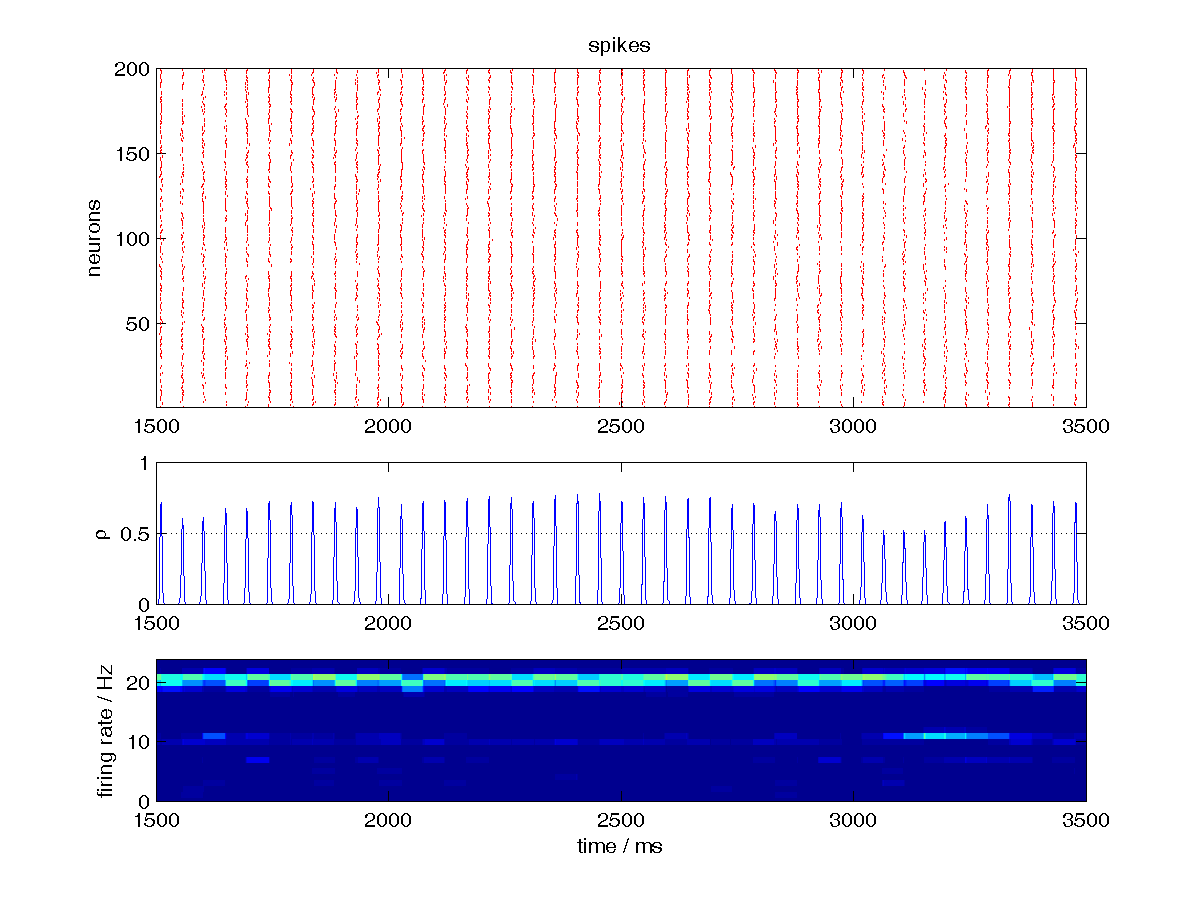
\includegraphics[scale=0.35]{fs-network-mean-in-phase.png}
        \caption{同相位状态。}
    \end{subfigure}
    \begin{subfigure}{0.45\textwidth}
        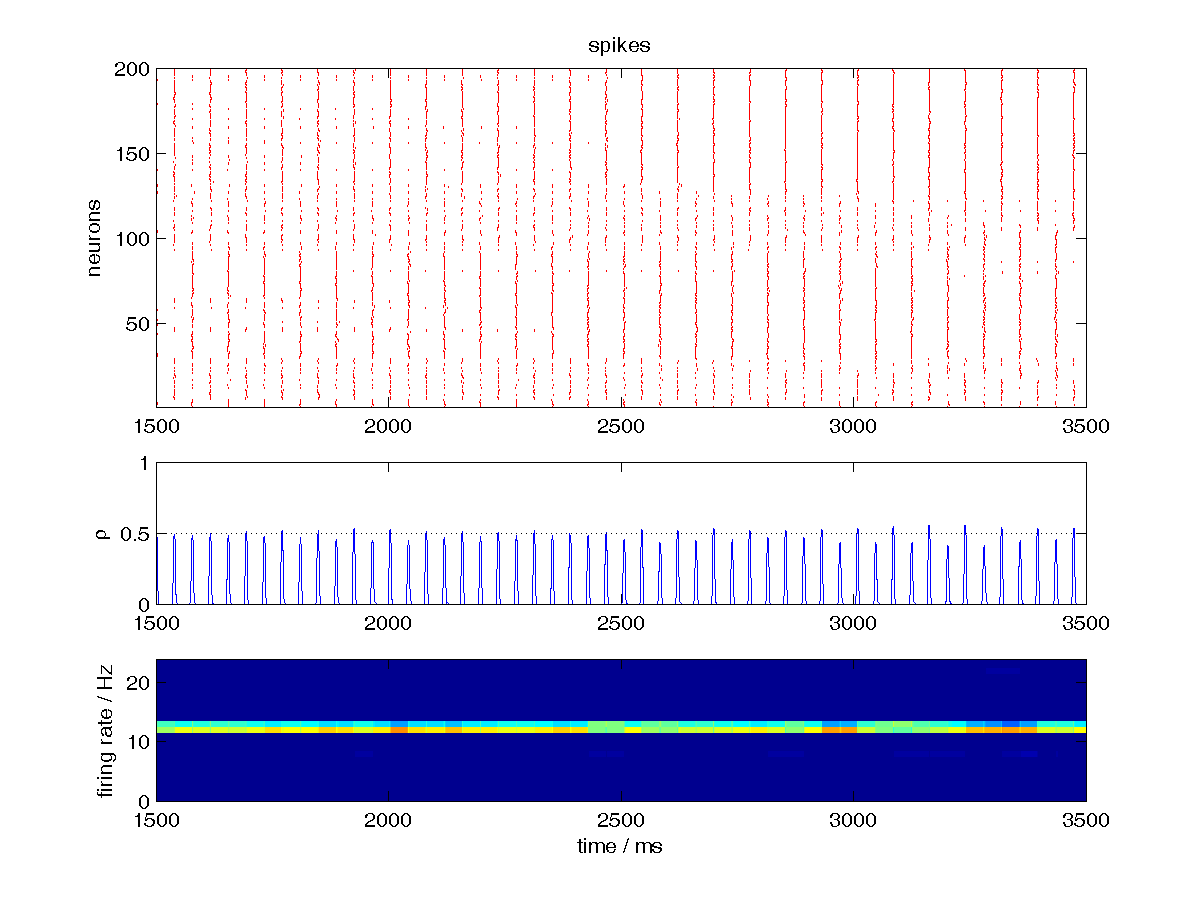
\includegraphics[scale=0.35]{fs-network-mean-anti-phase.png}
        \caption{反相位状态。}
    \end{subfigure}
    \begin{subfigure}{0.45\textwidth}
        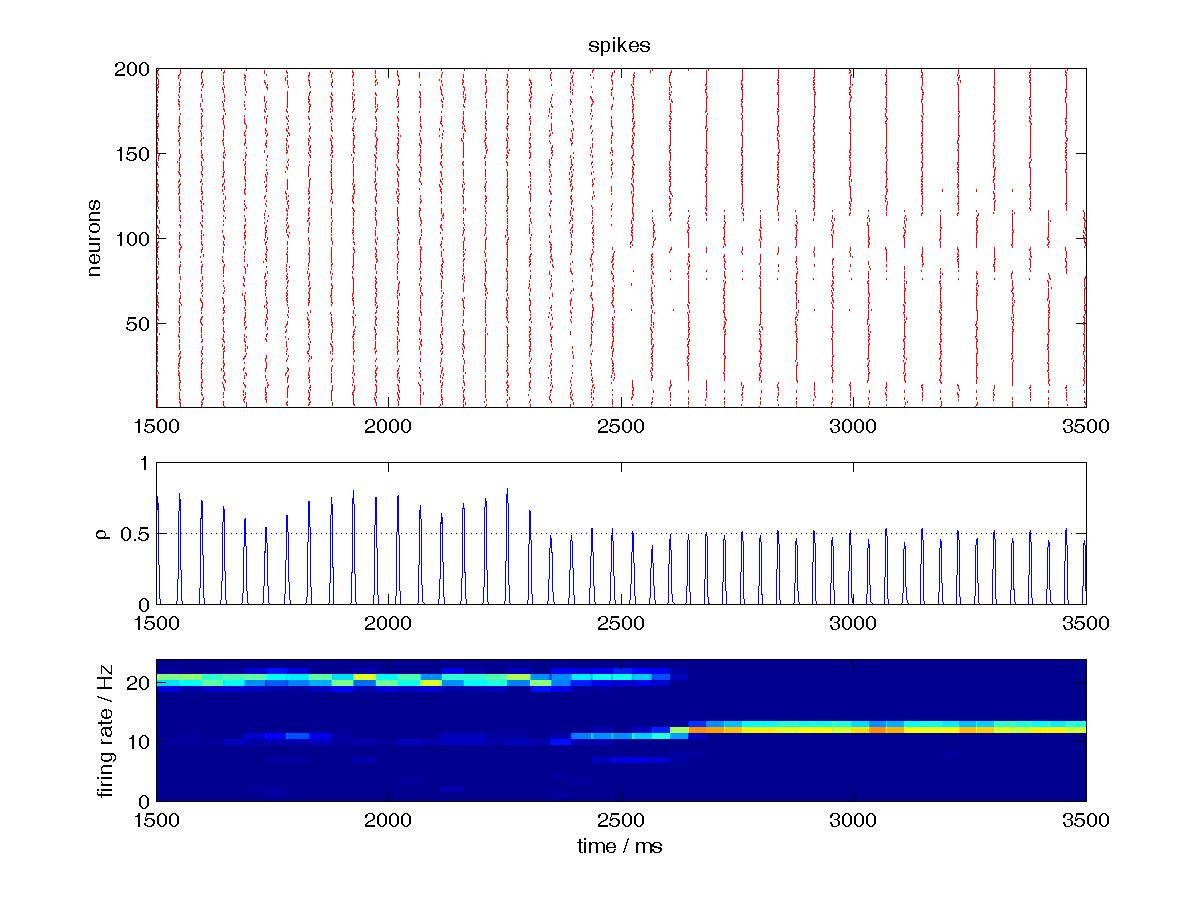
\includegraphics[scale=0.35]{fs-network-mean-transition.png}
        \caption{由同相位转移至反相位。}
    \end{subfigure}
    \begin{subfigure}{0.45\textwidth}
        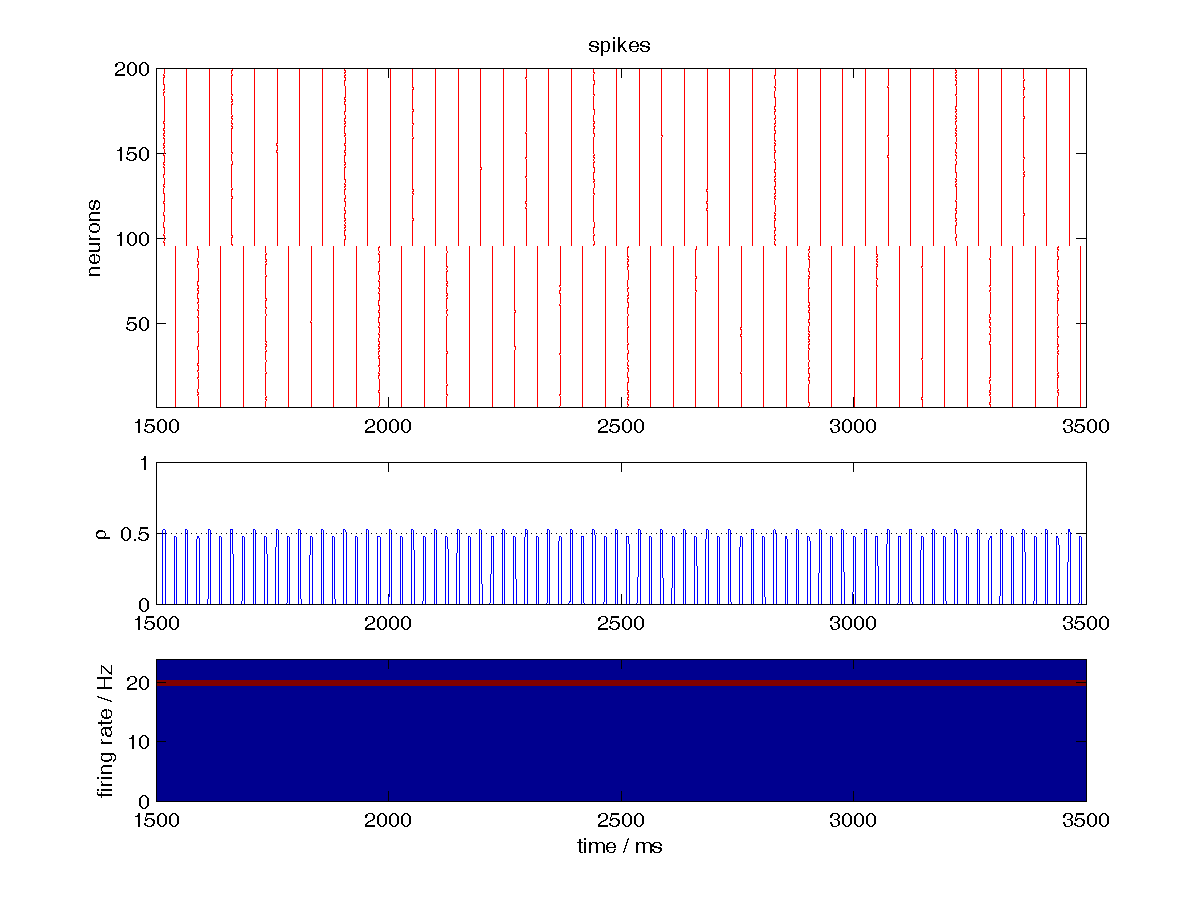
\includegraphics[scale=0.35]{fs-network-mean-block-async.png}
        \caption{没有非同步释放时的网络状态。}
    \end{subfigure}
\caption{网络的两种稳定状态。
背景电流输入为高斯,平均值$I_{\mu} = 80$ pA,$\dd{t} = 0.05$ ms。
非同步释放使用没有随机性的简化模型。
所有仿真计算中神经元和突触使用相同的随机初始状态。
为了使结果更清晰,神经元的编号经过了重新排列。
(a) 背景输入噪声很小 ($I_{\sigma} = 2.4$ pA),网络能够稳定在同相位状态。
(b) 背景噪声增大($I_{\sigma} = 3.2$ pA),网络只能处于反相位状态。
(c) 背景噪声适中($I_{\sigma} = 2.72$ pA),网络能在同相位状态稳定一段时间,之后进入反相位状态。没有观察到网络再回到同相位状态,可能是模拟的时间不够长。
(d) 没有非同步释放时($U_{ar} = 0$),网络进入反相位状态,此时背景噪声很小($I_{\sigma} = 2.4$ pA).}
\label{figure:network-stability}
\end{figure}

\paragraph{使用两个神经元的回路和相位反应曲线进行结果分析}
这里主要分析衰减常数的影响,于是把非同步释放替换为同步释放和衰减较慢的递质接收器。

在两个神经元的回路中,神经元 $\alpha$ 和神经元 $\beta$ 相互连接,没有自连接。背景噪声为高斯,具有相同的平均值和方差。
当两个神经元同步时,在第 $n$ 个周期
\begin{align}
\psi_{\alpha}\left(t\right) &= \left(\phi\left(t\right) + \phi_{\alpha}\left(n\right)\right) \mod 1 \\
\psi_{\beta}\left(t\right) &= \left(\phi\left(t\right) + \phi_{\beta}\left(n\right)\right) \mod 1
\end{align}
其中 $\phi\left(t\right) \in [0,1)$ 为周期函数。

那么两个神经元在第 $n$ 个周期的相位差为
\begin{equation}
\Delta\psi\left(n\right) = \left(\phi_{\alpha}\left(n\right) - \phi_{\beta}\left(n\right)\right) \mod 1
\end{equation}

假设经过一次交互,两个神经元的相位变化不大,且 $f\left(\phi\right)$ 是相位反应曲线,那么 $\alpha$ 的相位延迟为 $f(\Delta\psi\left(n\right))$, $\beta$ 的相位延迟为 $f(1-\Delta\psi\left(n\right))$。

那么在下一个周期,两者的相位差将是
\begin{equation}
\Delta\psi\left(n+1\right) = \left( \Delta\psi\left(n\right) + f(\Delta\psi\left(n\right)) - f(1-\Delta\psi\left(n\right)) \right) \mod 1
\end{equation}

因此,从 $g\left(\Delta\psi\right) = f(\Delta\psi) - f(1-\Delta\psi)$ 中我们可以推测相位差 $\Delta\psi\left(n\right)$ 的稳定性(见图\ref{figure:circuit-anti-phase-in-phase})。

\begin{figure}
    \begin{subfigure}{0.5\textwidth}
        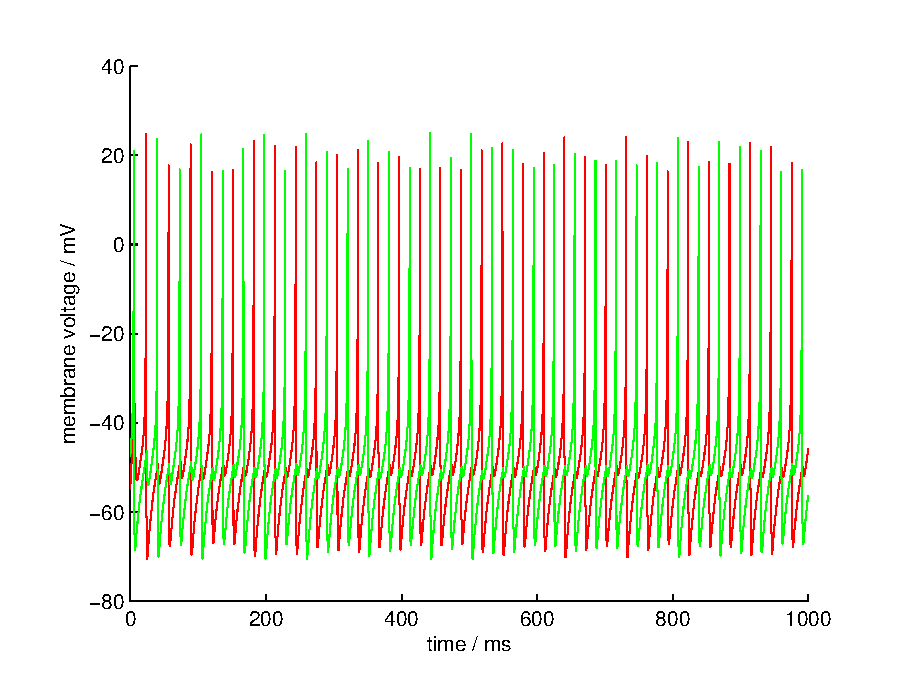
\includegraphics[scale=0.5]{fs-circuit-in-phase-unstable.eps}
        \caption{反相位状态。}
    \end{subfigure}
    \begin{subfigure}{0.5\textwidth}
        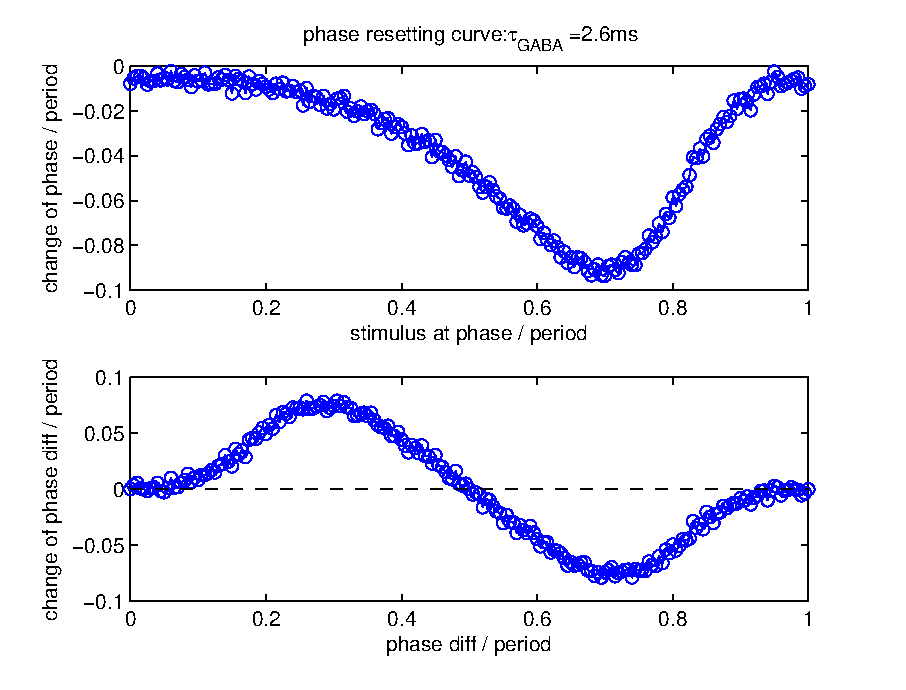
\includegraphics[scale=0.5]{fs-phase-resetting-fast-decay.eps}
        \caption{相位反应曲线。}
    \end{subfigure}
    \begin{subfigure}{0.5\textwidth}
        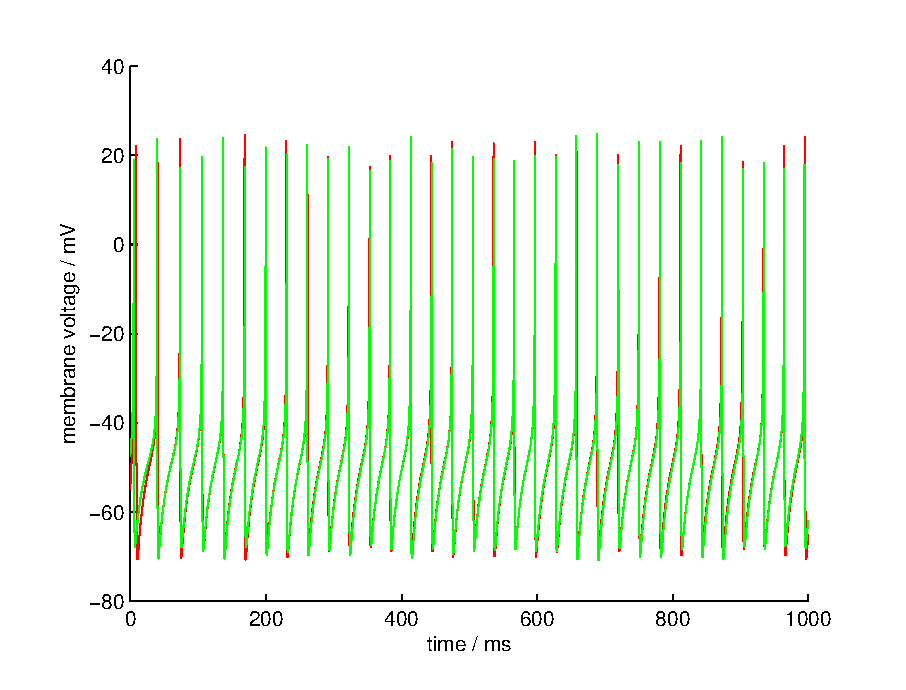
\includegraphics[scale=0.5]{fs-circuit-in-phase-stable.eps}
        \caption{同相位状态。}
    \end{subfigure}
    \begin{subfigure}{0.5\textwidth}
        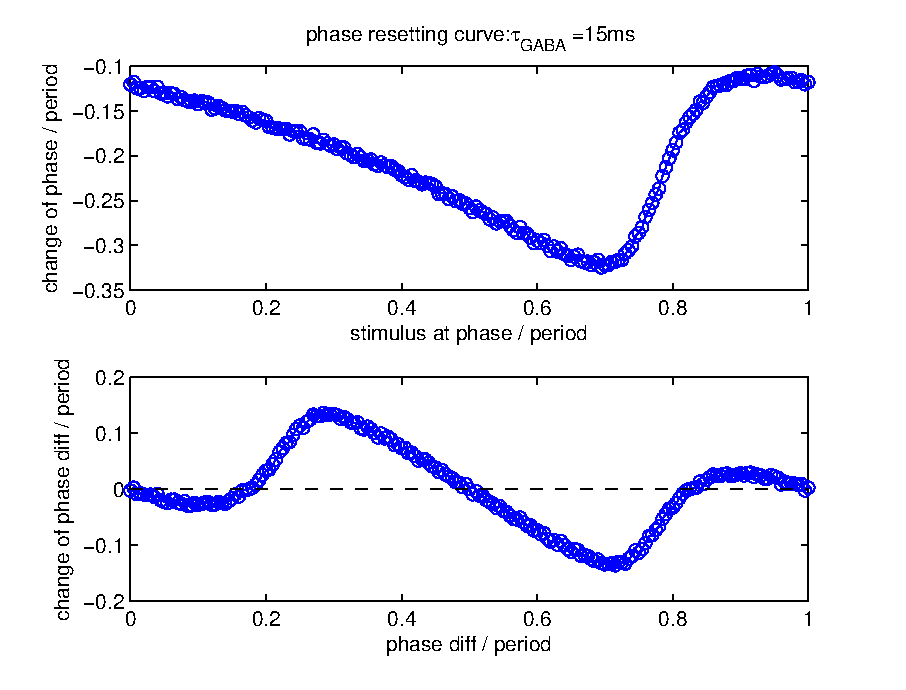
\includegraphics[scale=0.5]{fs-phase-resetting-slow-decay.eps}
        \caption{相位反应曲线。}
    \end{subfigure}
\caption{GABA 衰减常数较小时同相位状态不稳定,较大时同相位状态稳定。
(a) 两个神经元(红色和蓝色)通过 GABA 突触相连。$\tau_\text{GABA} = 2.6$ ms, $w_0 = 40$ nS。背景电流为高斯,平均值为 $I_{\mu} = 100$ pA ,标准差为 $I_{\sigma} = 3$ pA, $\dd{t} = 0.05$ ms。
(b) 对应于(a)中的神经元,上图为相位反应曲线 $f\left(\psi\right)$。下图为 $g\left(\Delta\psi\right)$。可以看出,唯一的稳定点为 $0.5$ 周期。测量相位反应曲线时,$w_{GABA} = 1$ nS。背景电流为常数 $I_{\mu} = 100$ pA, $\dd{t} = 0.005$ ms。
(c) 两个神经元(红色和蓝色)的参数变为 $\tau_\text{GABA} = 15$ ms, $w_0 = 10$ nS。背景电流为高斯,平均值为 $I_{\mu} = 100$ pA ,标准差为 $I_{\sigma} = 3$ pA, $\dd{t} = 0.05$ ms。
(d) 对应于(c),可以看出两个稳定点,分别为 $0$ 和 $0.5$ 周期。测量相位反应曲线时,$w_{GABA} = 1$ nS。背景电流为常数 $I_{\mu} = 100$ pA, $\dd{t} = 0.005$ ms。}
\label{figure:circuit-anti-phase-in-phase}
\end{figure}

非同步递质释放作为一个缓慢衰减的过程,可以使网络更容易稳定在同相位状态。

\subsection{非同步释放对网络发放精确性的影响}
\label{section:result:network-spike-timing}
非同步释放作为一种随机性释放,可能会使网络中神经元发放精确性降低。
基于每个神经元的发放间隔时间统计网络发放的时间精确性。
背景电流 $I_{\mu} = 100$ pA,没有噪声。网络一直处于反相位状态,网络整体发放频率随时间保持稳定。所以方差主要来自神经元之间的差异。

网络采用 $n = 200$ 个神经元,$\tau_\text{GABA} = 5$ ms, $w_0 = 35$ nS, $x_0 / X_F = 0.01$。

仿真计算结果显示更强的非同步释放能导致发放间隔的标准差变大。但影响大小取决于网络连接概率。
虽然突触有随机性,但当网络连接较密时,多个突触对同一个神经元的输入的随机性会相互抵消,所以总体随机性变小,而连接较稀疏时,随机性难以抵消,总体随机性较大(图\ref{figure:spike-timing-precision})。

非同步释放的增强可能有去同步的效果,但来自释放随机性的影响大小取决于网络连接的疏密程度。对于稠密的网络连接,释放随机性的影响较小(图\ref{figure:spike-timing-precision})。

\begin{figure}[H]
    \begin{subfigure}{0.5\textwidth}
        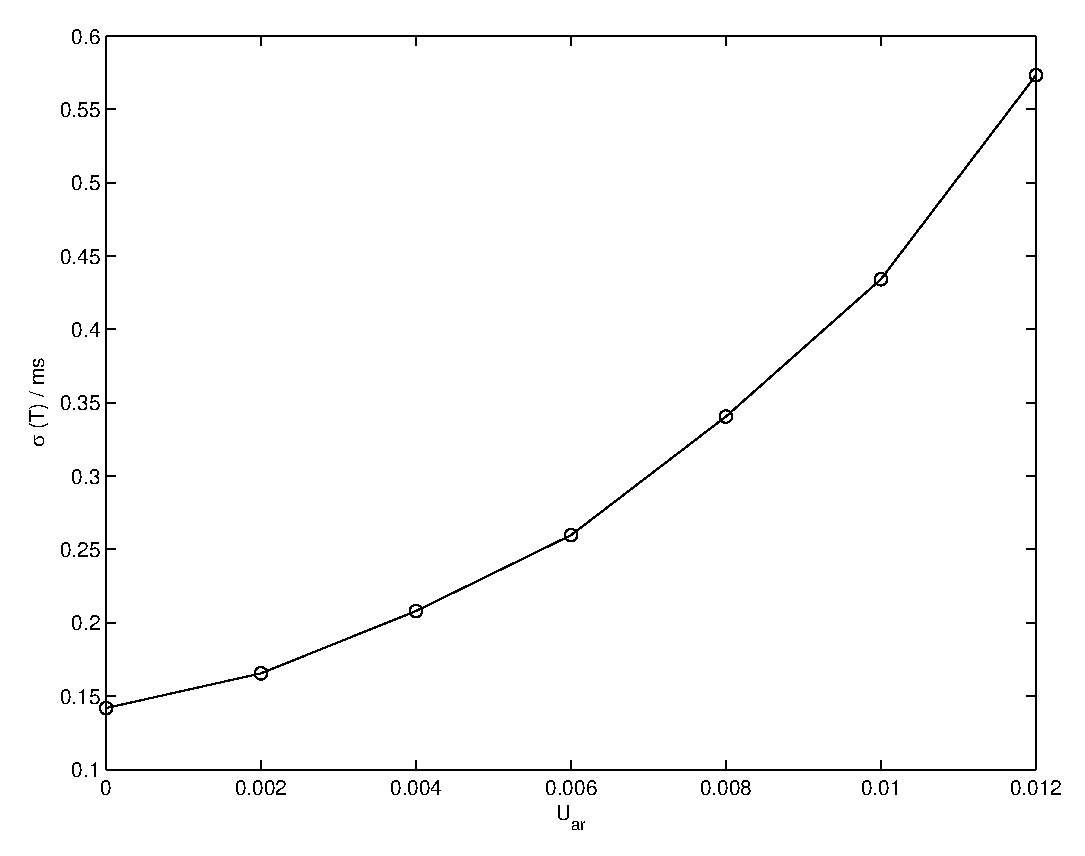
\includegraphics[scale=0.4]{fs-network-spike-timing-std-dense.eps}
        \caption{稠密连接网络中的效果。}
    \end{subfigure}
    \begin{subfigure}{0.5\textwidth}
        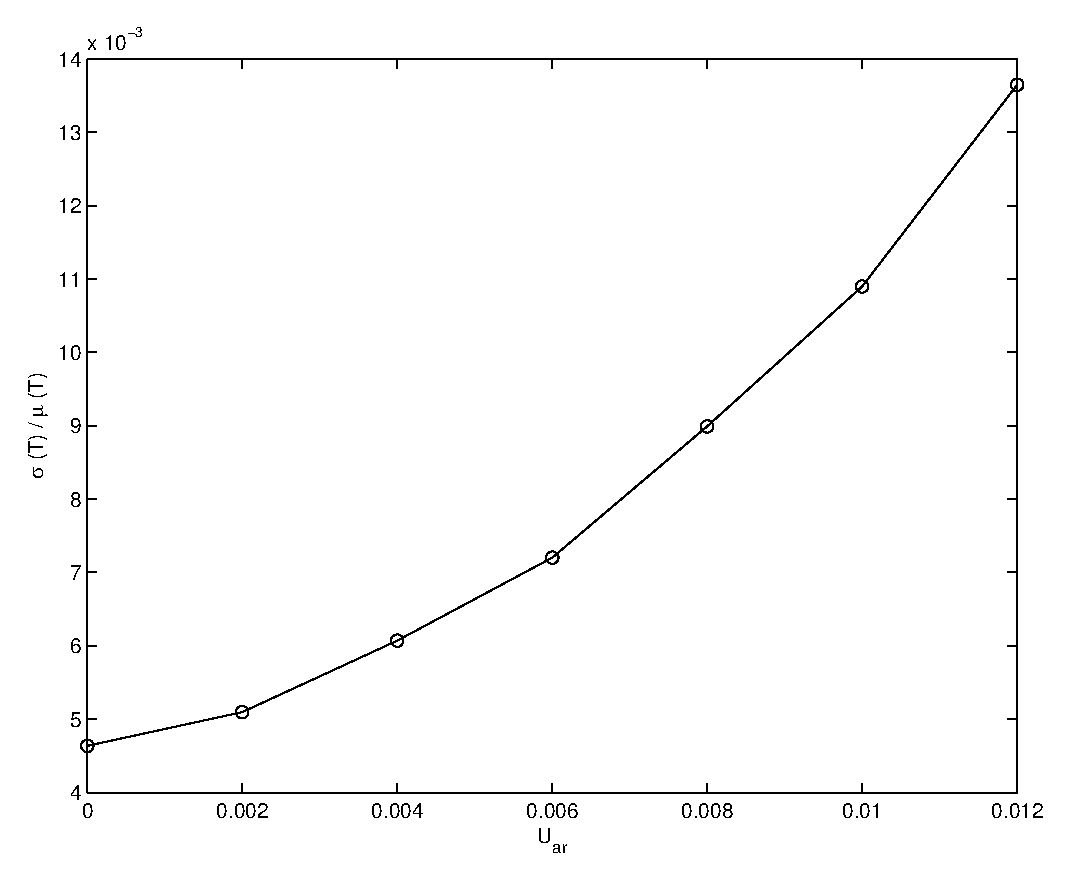
\includegraphics[scale=0.4]{fs-network-spike-timing-relative-dense.eps}
        \caption{稠密连接网络中的相对效果。}
    \end{subfigure}
    \begin{subfigure}{0.5\textwidth}
        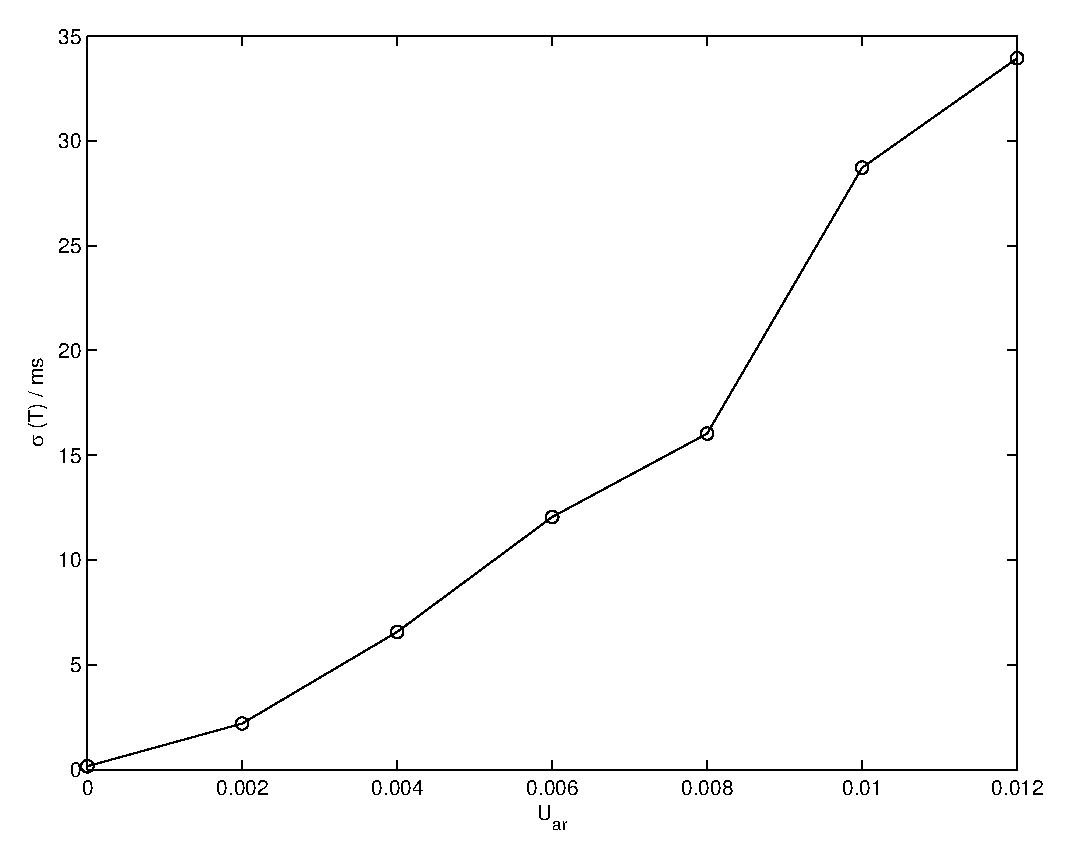
\includegraphics[scale=0.4]{fs-network-spike-timing-std-sparse.eps}
        \caption{稀疏连接网络中的效果。}
    \end{subfigure}
    \begin{subfigure}{0.5\textwidth}
        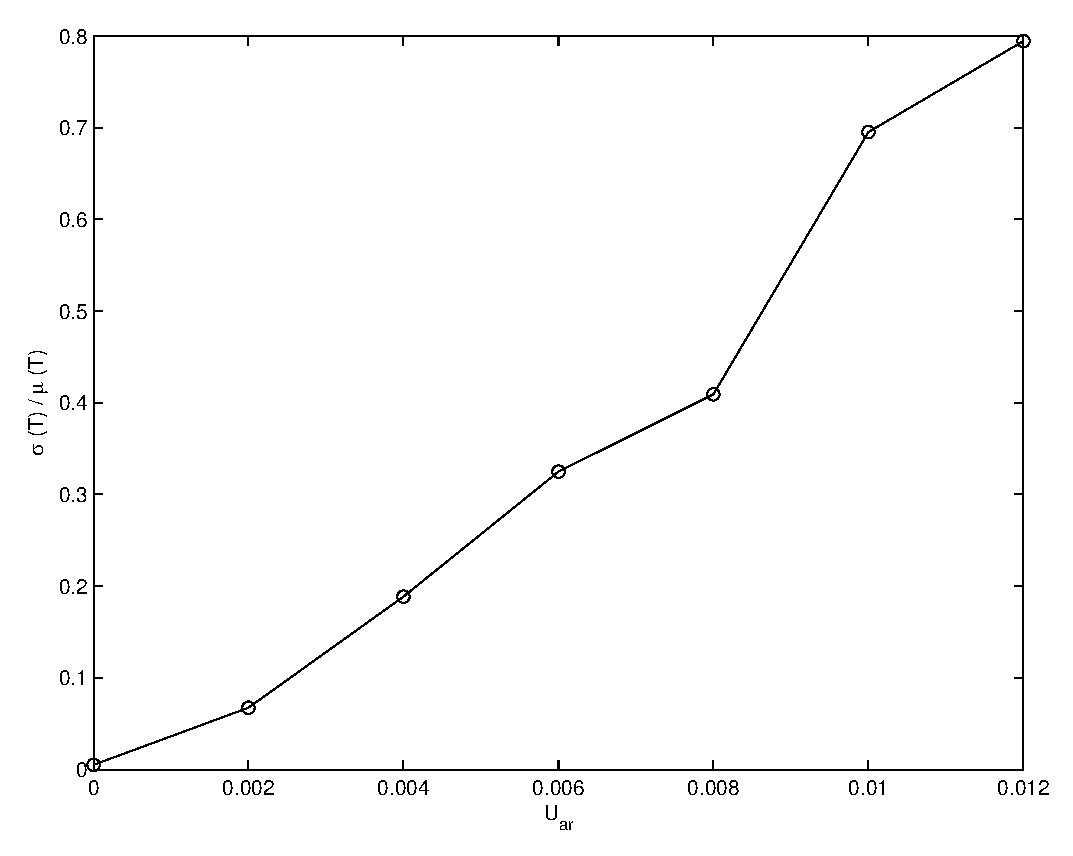
\includegraphics[scale=0.4]{fs-network-spike-timing-relative-sparse.eps}
        \caption{稀疏连接网络中的相对效果。}
    \end{subfigure}
\caption{更强的非同步释放使得神经元发放的时间更不精确。
(a) 发放间隔的标准差 $\sigma(T)$ 随非同步释放的增大(增大 $U_\text{ar}$ )而增大。链接概率为 $p = 1$。
(b) 相对值 $\sigma(T)/\mu(T)$ 也随非同步释放的增大而增大。连接概率为 $p = 1$。
(c) 发放间隔的标准差 $\sigma(T)$ 随非同步释放的增大(增大 $U_\text{ar}$ )而增大。链接概率为 $p = 0.3$。
(d) 相对值 $\sigma(T)/\mu(T)$ 也随非同步释放的增大而增大。连接概率为 $p = 0.3$。
统计使用刺激开始后第 $2$ s 到第 $4$ s 的发放间隔。背景电流为常数 $I_{\mu} = 100$ pA, $\dd{t} = 0.005$ ms。初始状态为随机生成,不同实验中都相同。}
\label{figure:spike-timing-precision}
\end{figure}

\subsection{非同步释放对网络自身的抑制性}
\label{section:result:network-self-inhibition}
网络选用 $n = 200$ 个神经元,$\tau_\text{GABA} = 2.6$ ms,链接概率 $p = 0.3$,$w_0 = 40$ nS。

在突触模型中, IPSC 依赖递质释放率和突触后细胞的细胞膜电位。
在同步发放的网络中,递质释放率与细胞膜膜电位高度相关,所以不能仅仅用 GABA 释放率来度量。
这里我们用网络平均发放频率来度量抑制性效果。

结果显示同步释放的增大(增大 $U_\text{sr}$)对网络抑制效果的影响不如非同步释放的增大(增大 $U_\text{ar}$),网络同步后抑制性主要由非同步释放提供(图\ref{figure:network-recurrent-inhibition})。

\begin{figure}
    \begin{subfigure}{0.5\textwidth}
        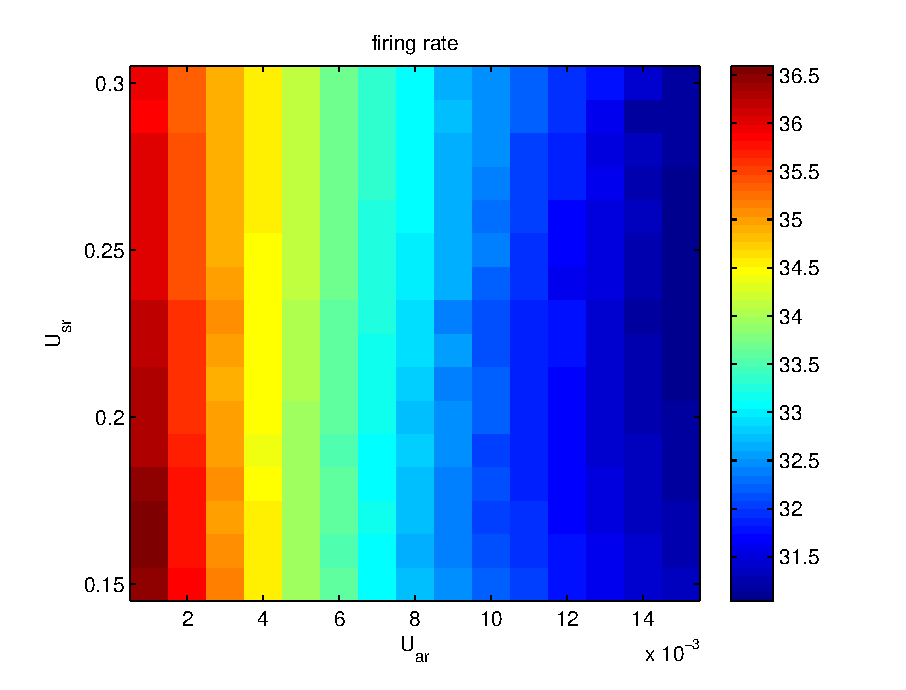
\includegraphics[scale=0.5]{fs-network-stat-u-firing-high-fast.eps}
        \caption{强背景电流。}
    \end{subfigure}
    \begin{subfigure}{0.5\textwidth}
        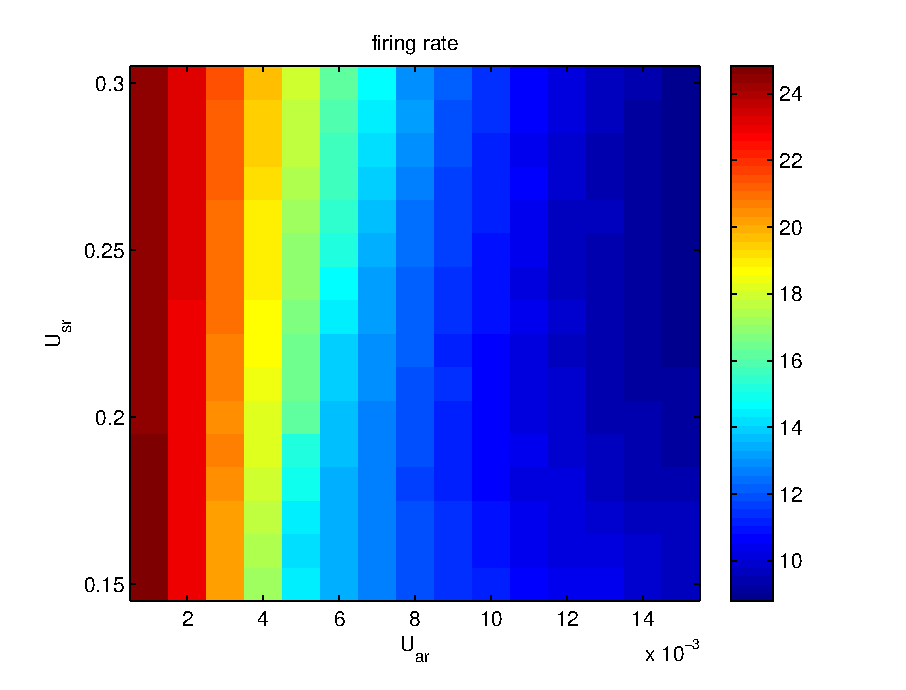
\includegraphics[scale=0.5]{fs-network-stat-u-firing-low-fast.eps}
        \caption{中等背景电流。}
    \end{subfigure}
\caption{同步释放和非同步释放对网络自身 抑制性的影响。
(a) 背景电流为高斯,平均值为 $I_{\mu} = 100$ pA ,标准差为 $I_{\sigma} = 3$ pA。
(b) 背景电流为高斯,平均值为 $I_{\mu} = 80$ pA ,标准差为 $I_{\sigma} = 2.4$ pA。
$\dd{t} = 0.05$ ms。}
\label{figure:network-recurrent-inhibition}
\end{figure}

\paragraph{用单神经元自抑制模型来分析原理}
为了分析网络行为的原理,我们用单个神经元来近似同步发放下的网络。
但个神经元有到自身的突触。
类似地,我们用不同递质接收器衰减常数的模型来分别近似同步释放和非同步释放。

如果固定突触权重,更高的 $\tau_\text{GABA}$ 会导致更高的平均电导。
\begin{equation}
\begin{split}
g_{mean} &= \frac{1}{T} \int_{0}^{T} {g_{GABA}\left(t\right)\dd{t}} \\
& \approx \frac{1}{T} \int_{0}^{\infty} {w \cdot \exp\left(-\frac{t}{\tau_\text{GABA}}\right)\dd{t}} \\
&= \frac{w\cdot \tau_\text{GABA}}{T}
\end{split}
\end{equation}
所以,为了使平均电导相同,我们将把 $w_{GABA}$ 根据 $\tau_\text{GABA}$ 进行归一化。

$Q_{GABA}$ 可以看作是加权求和的结果, $g\left(t\right)$ 则是每一时刻的权重。 $v\left(t\right) - E_{GABA}$ 随时间 $t$ 单调递增,所以更大的 $\tau{GABA}$ 使得权重分布偏向更大的 $v\left(t\right) - E_{GABA}$,这就导致 $Q_{GABA}$ 变大。
由于 $v\left(t\right) - E_{GABA}$ 在一个周期内变化巨大,所以权重的偏移能使 $Q_{GABA}$ 明显变化(见图\ref{figure:fs-neuron-tau-charge})。 

\begin{figure}
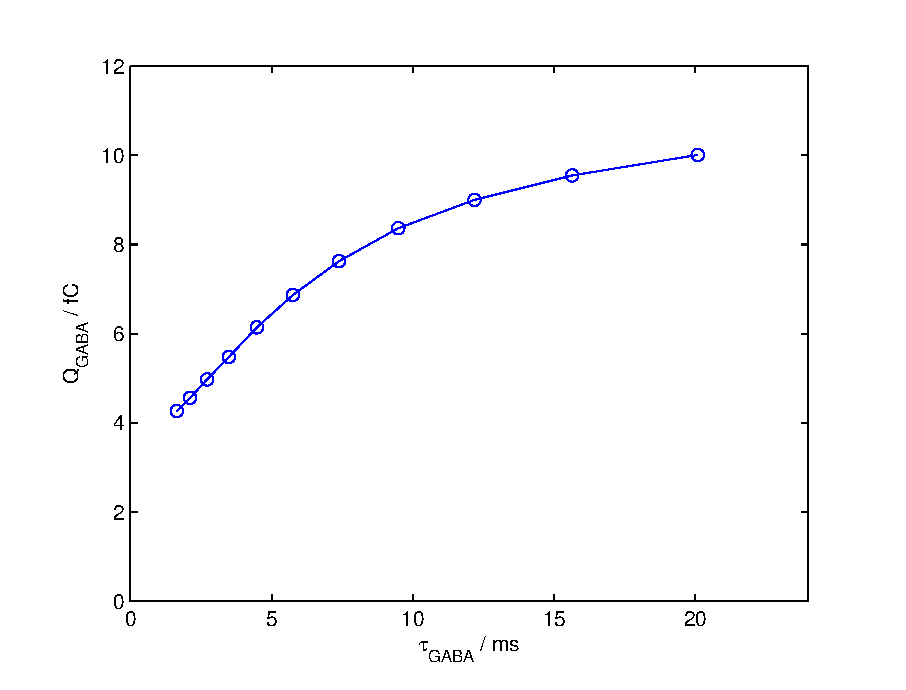
\includegraphics{fs-charge-tau-relation.eps}
\caption{每个周期内的 GABA 电量随 $\tau_\text{GABA}$ 的增大而增大。
突触权重进行了归一化,使得 $w \cdot \tau_\text{GABA} = w_{std} \cdot \tau_{std}$, $w_{std} = 1$ nS, $\tau_{std} = 5$ ms。
背景电流 $I_{\mu} = 100$ pA。
每个 $\tau_\text{GABA}$ 对应的突触权重都非常小,所以不会对发放周期有太大影响。}
\label{figure:fs-neuron-tau-charge}
\end{figure}

统计发放率来比较抑制性也得到了类似的结果(图\ref{figure:fs-neuron-inhibition})。

\begin{figure}
    \begin{subfigure}{0.5\textwidth}
        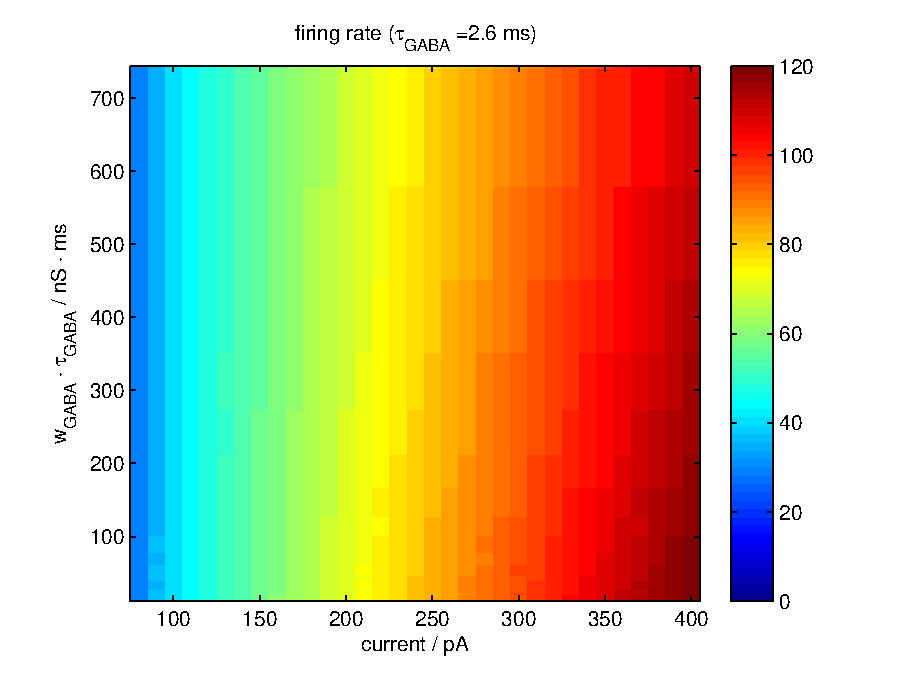
\includegraphics[scale=0.5]{fs-recurrent-input-output-fast-decay-normalized.eps}
        \caption{快速抑制。}
    \end{subfigure}
    \begin{subfigure}{0.5\textwidth}
        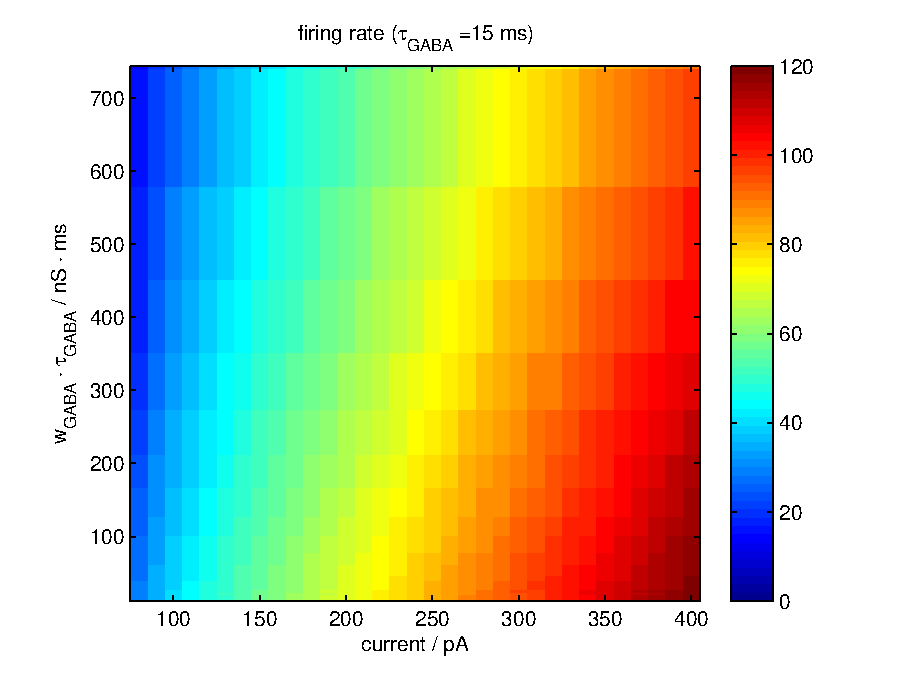
\includegraphics[scale=0.5]{fs-recurrent-input-output-slow-decay-normalized.eps}
        \caption{慢速抑制。}
    \end{subfigure}
\caption{不同 $\tau_\text{GABA}$ 下的输入输出关系。
(a) 当 $\tau_{GABA} = 2.6$ ms 较小时,增大权重对抑制性的影响较小。
(b) 当 $\tau_{GABA} = 15$ ms 较大时,增大权重对抑制性的影响较大。}
\label{figure:fs-neuron-inhibition}
\end{figure}

\chapter{讨论}
\label{chapter:discussion}


%%% 其它部分
\backmatter

% 本科生要这几个索引,研究生不要。选择性留下。
\makeatletter
\ifthu@bachelor
  % 插图索引
  %\listoffigures
  % 表格索引
  %\listoftables
  % 公式索引
  %\listofequations
\fi
\makeatother


% 参考文献
\bibliographystyle{thubib}
\bibliography{ref/refs}


% 致谢
%%% Local Variables:
%%% mode: latex
%%% TeX-master: "../main"
%%% End:

\begin{ack}
  衷心感谢导师 xxx 教授和物理系 xxx 副教授对本人的精心指导。他们的言传身教将使
  我终生受益。

  在美国麻省理工学院化学系进行九个月的合作研究期间,承蒙 xxx 教授热心指导与帮助,不
  胜感激。感谢 xx 实验室主任 xx 教授,以及实验室全体老师和同学们的热情帮助和支
  持!本课题承蒙国家自然科学基金资助,特此致谢。

  感谢 \thuthesis,它的存在让我的论文写作轻松自在了许多,让我的论文格式规整漂亮了
  许多。
\end{ack}


% 附录
\begin{appendix}
%%%% Local Variables: 
%%% mode: latex
%%% TeX-master: "../main"
%%% End: 

\chapter{外文资料原文}
\label{cha:engorg}
As one of the most widely used techniques in operations research, {\em
  mathematical programming} is defined as a means of maximizing a quantity known
as {\em objective function}, subject to a set of constraints represented by
equations and inequalities. Some known subtopics of mathematical programming are
linear programming, nonlinear programming, multiobjective programming, goal
programming, dynamic programming, and multilevel programming$^{[1]}$.

It is impossible to cover in a single chapter every concept of mathematical
programming. This chapter introduces only the basic concepts and techniques of
mathematical programming such that readers gain an understanding of them
throughout the book$^{[2,3]}$.


\section{Single-Objective Programming}
The general form of single-objective programming (SOP) is written
as follows,
\begin{equation}\tag*{(123)} % 如果附录中的公式不想让它出现在公式索引中,那就请
                             % 用 \tag*{xxxx}
\left\{\begin{array}{l}
\max \,\,f(x)\\[0.1 cm]
\mbox{subject to:} \\ [0.1 cm]
\qquad g_j(x)\le 0,\quad j=1,2,\cdots,p
\end{array}\right.
\end{equation}
which maximizes a real-valued function $f$ of
$x=(x_1,x_2,\cdots,x_n)$ subject to a set of constraints.

\newtheorem{mpdef}{Definition}[chapter]
\begin{mpdef}
In SOP, we call $x$ a decision vector, and
$x_1,x_2,\cdots,x_n$ decision variables. The function
$f$ is called the objective function. The set
\begin{equation}\tag*{(456)} % 这里同理,其它不再一一指定。
S=\left\{x\in\Re^n\bigm|g_j(x)\le 0,\,j=1,2,\cdots,p\right\}
\end{equation}
is called the feasible set. An element $x$ in $S$ is called a
feasible solution.
\end{mpdef}

\newtheorem{mpdefop}[mpdef]{Definition}
\begin{mpdefop}
A feasible solution $x^*$ is called the optimal
solution of SOP if and only if
\begin{equation}
f(x^*)\ge f(x)
\end{equation}
for any feasible solution $x$.
\end{mpdefop}

One of the outstanding contributions to mathematical programming was known as
the Kuhn-Tucker conditions\ref{eq:ktc}. In order to introduce them, let us give
some definitions. An inequality constraint $g_j(x)\le 0$ is said to be active at
a point $x^*$ if $g_j(x^*)=0$. A point $x^*$ satisfying $g_j(x^*)\le 0$ is said
to be regular if the gradient vectors $\nabla g_j(x)$ of all active constraints
are linearly independent.

Let $x^*$ be a regular point of the constraints of SOP and assume that all the
functions $f(x)$ and $g_j(x),j=1,2,\cdots,p$ are differentiable. If $x^*$ is a
local optimal solution, then there exist Lagrange multipliers
$\lambda_j,j=1,2,\cdots,p$ such that the following Kuhn-Tucker conditions hold,
\begin{equation}
\label{eq:ktc}
\left\{\begin{array}{l}
    \nabla f(x^*)-\sum\limits_{j=1}^p\lambda_j\nabla g_j(x^*)=0\\[0.3cm]
    \lambda_jg_j(x^*)=0,\quad j=1,2,\cdots,p\\[0.2cm]
    \lambda_j\ge 0,\quad j=1,2,\cdots,p.
\end{array}\right.
\end{equation}
If all the functions $f(x)$ and $g_j(x),j=1,2,\cdots,p$ are convex and
differentiable, and the point $x^*$ satisfies the Kuhn-Tucker conditions
(\ref{eq:ktc}), then it has been proved that the point $x^*$ is a global optimal
solution of SOP.

\subsection{Linear Programming} 
\label{sec:lp}

If the functions $f(x),g_j(x),j=1,2,\cdots,p$ are all linear, then SOP is called
a {\em linear programming}.

The feasible set of linear is always convex. A point $x$ is called an extreme
point of convex set $S$ if $x\in S$ and $x$ cannot be expressed as a convex
combination of two points in $S$. It has been shown that the optimal solution to
linear programming corresponds to an extreme point of its feasible set provided
that the feasible set $S$ is bounded. This fact is the basis of the {\em simplex
  algorithm} which was developed by Dantzig as a very efficient method for
solving linear programming.
\begin{table}[ht]
\centering
  \centering
  \caption*{Table~1\hskip1em This is an example for manually numbered table, which
    would not appear in the list of tables}
  \label{tab:badtabular2}
  \begin{tabular}[c]{|c|m{0.8in}|c|c|c|c|c|}\hline
    \multicolumn{2}{|c|}{Network Topology} & \# of nodes & 
    \multicolumn{3}{c|}{\# of clients} & Server \\\hline
    GT-ITM & Waxman Transit-Stub & 600 &
    \multirow{2}{2em}{2\%}& 
    \multirow{2}{2em}{10\%}& 
    \multirow{2}{2em}{50\%}& 
    \multirow{2}{1.2in}{Max. Connectivity}\\\cline{1-3}
    \multicolumn{2}{|c|}{Inet-2.1} & 6000 & & & &\\\hline
    \multirow{2}{1in}{Xue} & Rui  & Ni &\multicolumn{4}{c|}{\multirow{2}*{\thuthesis}}\\\cline{2-3}
    & \multicolumn{2}{c|}{ABCDEF} &\multicolumn{4}{c|}{} \\\hline
\end{tabular}  
\end{table}

Roughly speaking, the simplex algorithm examines only the extreme points of the
feasible set, rather than all feasible points. At first, the simplex algorithm
selects an extreme point as the initial point. The successive extreme point is
selected so as to improve the objective function value. The procedure is
repeated until no improvement in objective function value can be made. The last
extreme point is the optimal solution.

\subsection{Nonlinear Programming}

If at least one of the functions $f(x),g_j(x),j=1,2,\cdots,p$ is nonlinear, then
SOP is called a {\em nonlinear programming}.

A large number of classical optimization methods have been developed to treat
special-structural nonlinear programming based on the mathematical theory
concerned with analyzing the structure of problems.
\begin{figure}[h]
  \centering
  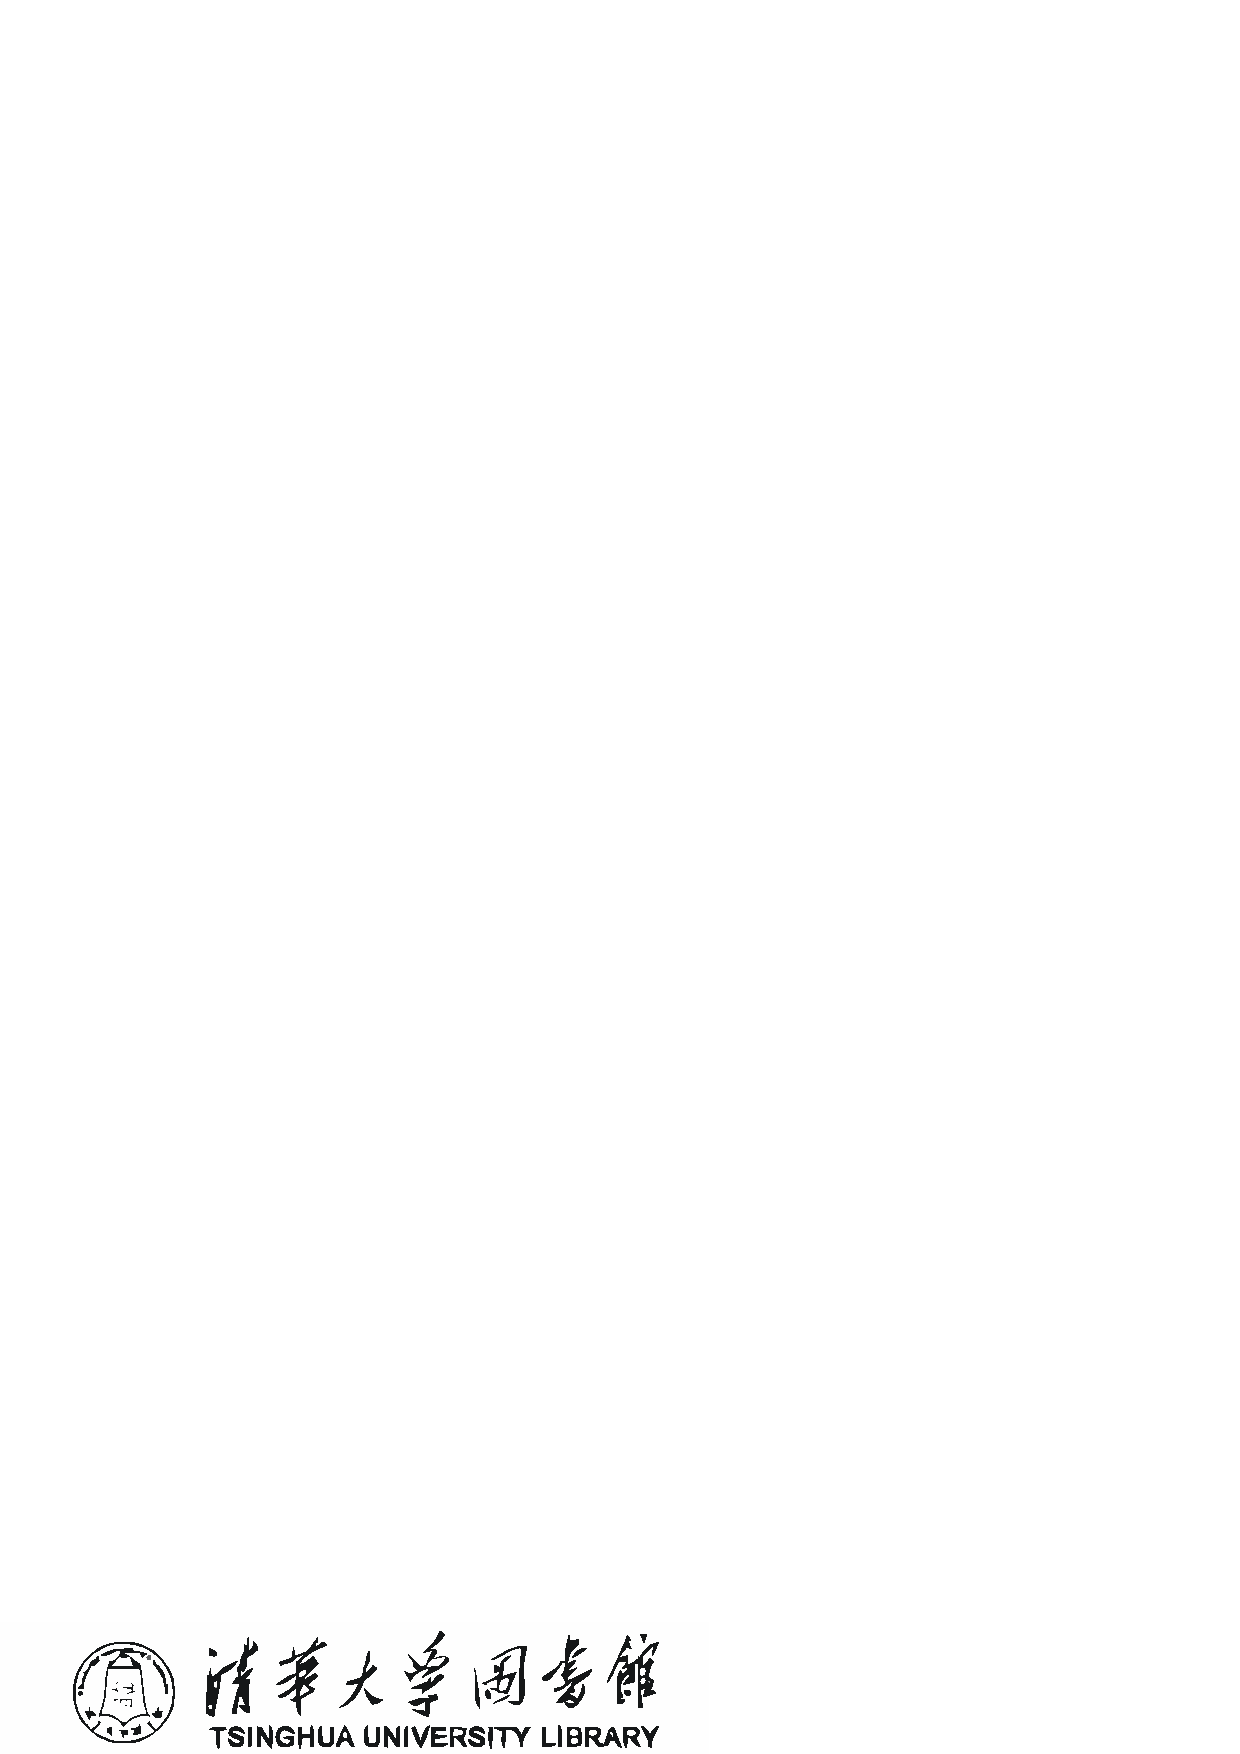
\includegraphics[clip]{thu-lib-logo}
  \caption*{Figure~1\hskip1em This is an example for manually numbered figure,
    which would not appear in the list of figures}
  \label{tab:badfigure2}    
\end{figure}

Now we consider a nonlinear programming which is confronted solely with
maximizing a real-valued function with domain $\Re^n$.  Whether derivatives are
available or not, the usual strategy is first to select a point in $\Re^n$ which
is thought to be the most likely place where the maximum exists. If there is no
information available on which to base such a selection, a point is chosen at
random. From this first point an attempt is made to construct a sequence of
points, each of which yields an improved objective function value over its
predecessor. The next point to be added to the sequence is chosen by analyzing
the behavior of the function at the previous points. This construction continues
until some termination criterion is met. Methods based upon this strategy are
called {\em ascent methods}, which can be classified as {\em direct methods},
{\em gradient methods}, and {\em Hessian methods} according to the information
about the behavior of objective function $f$. Direct methods require only that
the function can be evaluated at each point. Gradient methods require the
evaluation of first derivatives of $f$. Hessian methods require the evaluation
of second derivatives. In fact, there is no superior method for all
problems. The efficiency of a method is very much dependent upon the objective
function.

\subsection{Integer Programming}

{\em Integer programming} is a special mathematical programming in which all of
the variables are assumed to be only integer values. When there are not only
integer variables but also conventional continuous variables, we call it {\em
  mixed integer programming}. If all the variables are assumed either 0 or 1,
then the problem is termed a {\em zero-one programming}. Although integer
programming can be solved by an {\em exhaustive enumeration} theoretically, it
is impractical to solve realistically sized integer programming problems. The
most successful algorithm so far found to solve integer programming is called
the {\em branch-and-bound enumeration} developed by Balas (1965) and Dakin
(1965). The other technique to integer programming is the {\em cutting plane
  method} developed by Gomory (1959).

\hfill\textit{Uncertain Programming\/}\quad(\textsl{BaoDing Liu, 2006.2})

\section*{References}
\noindent{\itshape NOTE: these references are only for demonstration, they are
  not real citations in the original text.}

\begin{enumerate}[{$[$}1{$]$}]
\item Donald E. Knuth. The \TeX book. Addison-Wesley, 1984. ISBN: 0-201-13448-9
\item Paul W. Abrahams, Karl Berry and Kathryn A. Hargreaves. \TeX\ for the
  Impatient. Addison-Wesley, 1990. ISBN: 0-201-51375-7
\item David Salomon. The advanced \TeX book.  New York : Springer, 1995. ISBN:0-387-94556-3
\end{enumerate}

\chapter{外文资料的调研阅读报告或书面翻译}
\section{单目标规划}
北冥有鱼,其名为鲲。鲲之大,不知其几千里也。化而为鸟,其名为鹏。鹏之背,不知其几
千里也。怒而飞,其翼若垂天之云。是鸟也,海运则将徙于南冥。南冥者,天池也。 
\begin{equation}\tag*{(123)}
 p(y|\mathbf{x}) = \frac{p(\mathbf{x},y)}{p(\mathbf{x})}=
\frac{p(\mathbf{x}|y)p(y)}{p(\mathbf{x})}
\end{equation}

吾生也有涯,而知也无涯。以有涯随无涯,殆已!已而为知者,殆而已矣!为善无近名,为
恶无近刑,缘督以为经,可以保身,可以全生,可以养亲,可以尽年。

\subsection{线性规划}
庖丁为文惠君解牛,手之所触,肩之所倚,足之所履,膝之所倚,砉然响然,奏刀騞然,莫
不中音,合于桑林之舞,乃中经首之会。
\begin{table}[ht]
\centering
  \centering
  \caption*{表~1\hskip1em 这是手动编号但不出现在索引中的一个表格例子}
  \label{tab:badtabular3}
  \begin{tabular}[c]{|c|m{0.8in}|c|c|c|c|c|}\hline
    \multicolumn{2}{|c|}{Network Topology} & \# of nodes & 
    \multicolumn{3}{c|}{\# of clients} & Server \\\hline
    GT-ITM & Waxman Transit-Stub & 600 &
    \multirow{2}{2em}{2\%}& 
    \multirow{2}{2em}{10\%}& 
    \multirow{2}{2em}{50\%}& 
    \multirow{2}{1.2in}{Max. Connectivity}\\\cline{1-3}
    \multicolumn{2}{|c|}{Inet-2.1} & 6000 & & & &\\\hline
    \multirow{2}{1in}{Xue} & Rui  & Ni &\multicolumn{4}{c|}{\multirow{2}*{\thuthesis}}\\\cline{2-3}
    & \multicolumn{2}{c|}{ABCDEF} &\multicolumn{4}{c|}{} \\\hline
\end{tabular}  
\end{table}

文惠君曰:“嘻,善哉!技盖至此乎?”庖丁释刀对曰:“臣之所好者道也,进乎技矣。始臣之
解牛之时,所见无非全牛者;三年之后,未尝见全牛也;方今之时,臣以神遇而不以目视,
官知止而神欲行。依乎天理,批大郤,导大窾,因其固然。技经肯綮之未尝,而况大坬乎!
良庖岁更刀,割也;族庖月更刀,折也;今臣之刀十九年矣,所解数千牛矣,而刀刃若新发
于硎。彼节者有间而刀刃者无厚,以无厚入有间,恢恢乎其于游刃必有余地矣。是以十九年
而刀刃若新发于硎。虽然,每至于族,吾见其难为,怵然为戒,视为止,行为迟,动刀甚微,
謋然已解,如土委地。提刀而立,为之而四顾,为之踌躇满志,善刀而藏之。”

文惠君曰:“善哉!吾闻庖丁之言,得养生焉。”


\subsection{非线性规划}
孔子与柳下季为友,柳下季之弟名曰盗跖。盗跖从卒九千人,横行天下,侵暴诸侯。穴室枢
户,驱人牛马,取人妇女。贪得忘亲,不顾父母兄弟,不祭先祖。所过之邑,大国守城,小
国入保,万民苦之。孔子谓柳下季曰:“夫为人父者,必能诏其子;为人兄者,必能教其弟。
若父不能诏其子,兄不能教其弟,则无贵父子兄弟之亲矣。今先生,世之才士也,弟为盗
跖,为天下害,而弗能教也,丘窃为先生羞之。丘请为先生往说之。”
\begin{figure}[h]
  \centering
  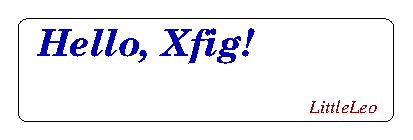
\includegraphics{hello}
  \caption*{图~1\hskip1em 这是手动编号但不出现索引中的图片的例子}
  \label{tab:badfigure3}    
\end{figure}

柳下季曰:“先生言为人父者必能诏其子,为人兄者必能教其弟,若子不听父之诏,弟不受
兄之教,虽今先生之辩,将奈之何哉?且跖之为人也,心如涌泉,意如飘风,强足以距敌,
辩足以饰非。顺其心则喜,逆其心则怒,易辱人以言。先生必无往。”

孔子不听,颜回为驭,子贡为右,往见盗跖。

\subsection{整数规划}
盗跖乃方休卒徒大山之阳,脍人肝而餔之。孔子下车而前,见谒者曰:“鲁人孔丘,闻将军
高义,敬再拜谒者。”谒者入通。盗跖闻之大怒,目如明星,发上指冠,曰:“此夫鲁国之
巧伪人孔丘非邪?为我告之:尔作言造语,妄称文、武,冠枝木之冠,带死牛之胁,多辞缪
说,不耕而食,不织而衣,摇唇鼓舌,擅生是非,以迷天下之主,使天下学士不反其本,妄
作孝弟,而侥幸于封侯富贵者也。子之罪大极重,疾走归!不然,我将以子肝益昼餔之膳。”


\chapter{其它附录}
前面两个附录主要是给本科生做例子。其它附录的内容可以放到这里,当然如果你愿意,可
以把这部分也放到独立的文件中,然后将其 \verb|\input| 到主文件中。
\end{appendix}

% 个人简历
%\begin{resume}
  \begin{enumerate}[{[}1{]}]
  \item Wang T\textsuperscript{1}, Yin L, Rasch MJ, Shu Y, Wu S\textsuperscript{*}. A Phenomenological Synapse Model for Asynchronous Neurotransmitter Release. {\it PLoS Computational Biology} (SCI 2区, 审稿中)
  \end{enumerate}

\end{resume}

\end{document}
